\documentclass[a4paper,12pt]{article}

\usepackage[a4paper]{geometry}
\usepackage{amssymb,amsmath}
\usepackage{amsthm}
\usepackage[utf8]{inputenc}
\usepackage{enumerate}
\usepackage{color}
\usepackage{graphicx}
\usepackage[estonian]{babel}
\usepackage[usenames,dvipsnames]{xcolor}
\usepackage{float}
\usepackage{cite}
\usepackage{etoolbox}
\usepackage{theoremref}
\usepackage[hidelinks]{hyperref}
\usepackage{tikz}
\usepackage{framed}
\usepackage[framemethod=tikz]{mdframed}
\usepackage{diagbox}
\usepackage{pifont}
\usepackage{colortbl}

\renewcommand\thefootnote{\ding{\numexpr171+\value{footnote}}}


\allowdisplaybreaks
\makeatletter
\patchcmd{\HyField@FlagsRadioButton}{\HyField@SetFlag{Ff}{Radio}}{}{}{}
\makeatother
\def\DefaultOptionsofRadio{print}



\definecolor{background_example}{HTML}{EDEDED}
%E0DCDE


\setlength\parindent{0pt}
\newenvironment{tightcenter}{%
  \setlength\topsep{0pt}
  \setlength\parskip{0pt}
  \begin{center}
}{%
  \end{center}
}
\newsavebox{\thisOne}
\newenvironment{meeldetuletus}{
	\begin{lrbox}{\thisOne}
		\begin{minipage}{0.95\textwidth} \vspace{0.25em} {\scriptsize \textsc{meeldetuletuseks}} \linebreak \vspace{-2em}
} 
{  
 \end{minipage}\end{lrbox}{
 		
 			\begin{mdframed}[tikzsetting={draw=black,dashed,line width=0.5pt, dash pattern = on 10pt off 3pt},%
 			linecolor=background_example,backgroundcolor=background_example,outerlinewidth=1pt]
 			\usebox{\thisOne}
 			\end{mdframed}
 		
 		
 	}
}
\newsavebox{\boxTwo}
\newenvironment{naide}{
    \begin{lrbox}{\boxTwo}
        \begin{minipage}{\textwidth}
    }
    {\end{minipage}\end{lrbox}
    	\colorbox{background_example}{\usebox{\boxTwo}}
    }

\author{Vootele Rõtov}
\title{Bakatöö}

\numberwithin{equation}{section}
\theoremstyle{definition}
\newtheorem*{elementaarsyndmus}{Definitsioon}
\newtheorem*{toenaosus}{Definitsioon}
\newtheorem*{juhuslik_suurus}{Definitsioon}
\newtheorem*{jaotus}{Definitsioon}
\newtheorem*{keskvaartus}{Definitsioon}
\newtheorem*{dispersioon}{Definitsioon}
\newtheorem{keskvaartus_konstant}[equation]{Lause}
\newtheorem{dispersioon_konstant}[equation]{Lause}
\newtheorem*{kovariatsioon}{Definitsioon}
\newtheorem*{korrelatsioon}{Definitsioon}
\newtheorem{summa_dispersioon}[equation]{Lause}
\newtheorem{summa_kovariatsioon}[equation]{Lause}
\newtheorem*{mittenegatiivselt_maaratud}{Definitsioon}
\newtheorem{konstant_kovariatsioon}[equation]{Lause}
\newtheorem{kumer_hulk}[equation]{Definitsioon}
\newtheorem{kumer_f}[equation]{Definitsioon}


\begin{document}

\maketitle

\pagebreak

\tableofcontents

\pagebreak

\section{Sissejuhatus}

Käesoleva bakalaureuse töö on saanud motivatsiooni psühholoogide praktilisest probleemist - kuidas hinnata nende töövaldkonnas tihti kasutatavate valikvastustega testide headust. Tuleb välja, et ühe testide headust kirjeldava karakteristiku - reliaabluse, hindamiseks sobivad vahendid saame klassikalise testiteooria (\textit{Classical Test Theory}) nimelise matemaatilise teooria tulemuste põhjal. 

Töö esimeses osas anname vajaliku taustinfo ja probleemipüstituse. Seejärel ehitame üles meile vajamineva osa klassikalisest testiteooriast - defineerime reliaabluse ning rajame vundamendi selle hindamiseks. Järgneval vaatleme erinevaid võimalusie reliaabluse hindamiseks. Lõpetuseks uurime põgusalt ühte võimalikku lähenemist järjestikskaala tõlgendamiseks intervallskaalana, mis kasutab ära eelnevalt uuritud reliaabluse hinnanguid ja sättestab tõlgendamis probleemi optimiseerimisprobleemina.

Töö eesmärgiks on anda eesti keelne ülevaade klassikalisest testiteooria alustest, mida autorile teadaolevalt ei ole käsitletud matemaatilisest aspektist vaadelduna - olemasolevad käsitlused on mõeldud praktiliseks abivahendiks psühholoogile ning seetõttu teistsuguse lähenemisega. Peale selle on töö eesmärgiks ka reliaabluse hindamiseks sobivate vahendite tutvustamine tasemel, millest võiks loodetavasti kasu olla ka teste koostavatele praktikutele. Uurimuse viimases osas loodame lugejale tutvustada tavapärasest teistsuguse lähenemist testi tulemuste kvantitiivsele tõlgendamisele, mis tugineb viimase aja edusammudele optimiseerimise valdkonnas.


Lisaks loetavale dokumendile on töö väljundiks ka teek, mis sisaldab funktsioone kõigi töös välja toodud hinnangute leidmiseks testi tulemuste põhjal ning leiab loodetavasti psühholoogide poolt kasutamist. 


\pagebreak



\section{Taustinfo ja probleemipüstitus}

Järgnevalt anname vajalikud taustateadmised probleemi mõtestamiseks ning peatüki lõpetuseks püstitame käesoleva töö kesksed probleemid.

\subsection{Küsimustik, küsimus ja Likerti skaala}

Käesolev uurimus tegeleb k\"usimustikega (\textit{Likert scale}), milles soovitakse hinnanguid teatud arvule küsimustele (\textit{Likert item}) $n$ pallisel Likerti skaalal \cite{Edmondson}, kus $n$ jääb enamasi kahe ja kümne vahele. Käsitleme Likerti skaalasid, mis on sümmeetrilised, see tähendab, et positiivsete ja negatiivsete vastuse variantide arv on sama. Näiteks:\footnote{Näited terviklikest k\"usimustikest on lisades, \hyperref[likert1]{joonisel \ref*{likert1}} ja \hyperref[likert2]{ \ref*{likert2}}}

\vspace{10pt}

\begin{figure}[H]


\colorbox{background_example}{\parbox{\textwidth}{

\vspace{1mm}

Käesoleva bakalaureusetöö \"ulesehitus on loogiline.

\vspace{5pt}

\begin{Form}
\def\DefaultWidthofChoiceMenu{12pt}%


\small{
	\CheckBox[bordercolor = gray,name=optionE]{\mbox{}} Ei nõustu 
	\CheckBox[bordercolor = gray,name=optionD]{\mbox{}} Ei nõustu osaliselt
	\CheckBox[bordercolor = gray,name=optionC]{\mbox{}} Nii ja naa
	\CheckBox[bordercolor = gray,name=optionC]{\mbox{}}  Nõustun osaliselt
	\CheckBox[checked,bordercolor = gray,name=optionC]{\mbox{}} Nõustun
}


\end{Form}}}
\caption{Näide väitest, millele palutakse hinnangut Likerti skaalal}
\label{likert_question}
\end{figure}

\subsection{Likerti skaala tõlgendamine intervallskaalana}

Likerti skaala tõlgendamisel intervallksaalana on väljakujunenud tava seada valikvastustele vastavusse järjestatud täisarvud, kusjuures mida posiitiivsem vastuseevariant, seda suurem temale vastavusse seatud arv. Reeglina kasutatakse kas arve alates ühest kuni valikvastuste arvuni või valitakse välja täisarvud nii, et neutraalsele vastusevariandile vastab null.

\begin{figure}[H]

\colorbox{background_example}{\parbox{\textwidth}{

\vspace{1mm}

Käesoleva bakalaureusetöö \"ulesehitus on loogiline.

\vspace{5pt}

\begin{tikzpicture}
\node at (0,0) {};
\draw[very thick, ->] (0.625em,0em) -- (0.625em,1.5em) node[label=above: -2] {};
\draw[very thick, ->] (6.375em,0em) -- (6.375em,1.5em) node[label=above: -1] {};
\draw[very thick, ->] (15.75em,0em) -- (15.75em,1.5em) node[label=above: 0] {};
\draw[very thick, ->] (21.625em,0em) -- (21.625em,1.5em) node[label=above: 1] {};
\draw[very thick, ->] (30.5em,0em) -- (30.5em,1.5em) node[label=above: 2] {};
\end{tikzpicture}

\begin{Form}
\def\DefaultWidthofChoiceMenu{12pt}%
\small{
\CheckBox[bordercolor = gray,name=optionE1]{\mbox{}} Ei nõustu 
\CheckBox[bordercolor = gray,name=optionD1]{\mbox{}} Ei nõustu osaliselt
\CheckBox[bordercolor = gray,name=optionC1]{\mbox{}} Nii ja naa
\CheckBox[checked,bordercolor = gray,name=optionC1]{\mbox{}}  Nõustun osaliselt
\CheckBox[bordercolor = gray,name=optionC1]{\mbox{}} Nõustun
}
\end{Form}



\begin{tikzpicture}
\node at (0,0) {};
\draw[very thick, ->] (0.625em,0em) -- (0.625em,-1.5em) node[label=below: 1] {};
\draw[very thick, ->] (6.375em,0em) -- (6.375em,-1.5em) node[label=below: 2] {};
\draw[very thick, ->] (15.75em,0em) -- (15.75em,-1.5em) node[label=below: 3] {};
\draw[very thick, ->] (21.625em,0em) -- (21.625em,-1.5em) node[label=below: 4] {};
\draw[very thick, ->] (30.5em,0em) -- (30.5em,-1.5em) node[label=below: 5] {};
\end{tikzpicture}}}
\caption{Näide kahest levinumast Likerti skaala tõlgendusest invtervallskaalana }
\label{likert_question}
\end{figure}

Lugejal võib tekkida õigustatud k\"usimus, kuidas põhjendab autor Likerti skaala käsitlemist intervallskaalana, kui Likerti skaala on olemuseslt järjestikskaala ning selle tõlgendamises intervallskaalana on vastuoluline küsimus, näiteks \cite{Jamieson2004}. Siinkohal tõdeme, et Likerti skaala tõlgendamine intervallksaalana on praktikas piisavalt levinud, et selle valdkonna uurimine õigustatud oleks - olenamat selle teoreetilisest põhjendatusest.  Siinkohal väärib autori silmis esile toomist kriitikute \"uks levinumaid argumente -  "`hea"'  ja "`väga hea"'  keskmine ei ole  loomulikul viisil tõlgendatav kui "`hea + pool"' ehk pole mingit põhjust eeldada, et kõikide küsimuste omavaheline kaugus on mingil põhjusel võrdne. Autor nõustub selle kriitikaga ning loodab töö neljandas osas pakkuda alternatiivse tõlgendusviisi. 



\subsection{Testi valiidsus}

Testi \textbf{valiidsus} on testi karakteristik, mis iseloomustab testi võimet mõõta seda, mida ta disainiti mõõtma. Enamikes käsitlustes vaadeltakse valiidsust kui väärtust intervall skaalal nulli ja ühe vahel.

Näitena, kaal mis näitab 75 kilo kaaluva inimese kaaluks 74,5 kilo omab kõrgemat valiidsust kui kaal, mis sama inimese puhul näitab kaaluks 65 kilo.   

Arusaadavatel põhjustel on testi valiidsus äärmiselt oluline ning psühholoogiliste testide valiidsuse hindamine on olnud üks psühhomeetria põhilistest uurimisobjektidest. Sellega seoses on palju tööd tehtud ka valiidsuse definitsiooni täpsemaks muutmisega, võrreldes selle paragrahvi alguses antud väga intuitiivse definitsiooniga. Kuna valiidsus on selle töö raames vajalik vaid taustinfona probleemi mõttestamisel tundub antud lihtne definitsioon aga sobivaim. 

\subsection{Testi reliaablus}

Testi \textbf{reliaablus} on testi omadust saada sama subjekti erinevatel mõõtmistel sama testiga sama tulemus ehk testi stabiilsus. Nagu valiidsus, on ka reliaablus reeglina määratud intervall skaalal, nulli ja ühe vahel. 

Näitena, kaal mis näitab 75 kilo kaaluva inimese kaaluks 74,5 kilo igal kaalumisel omab kõrgemat reliaablust kui kaal, mis näitab juhuslikult kas 74,5 kilo või 75,5 kilo. 

Reliaabluse täpsema, matemaatilise definitsioone anname edaspidi. 

\subsection{Valiidsuse ja reliaabluse suhe}

Valiidsuse ja reliaabluse suhestamisel kerkib kiiresti üles loomulik küsimus - kas test võib olla samaaegselt suure valiidsuse ja väikse reliaablusega? Eelpool antud definitsioonid jättavad selle küsimuse lahtiseks - vaatleme järgmist olukorda:

\begin{figure}[H]
\colorbox{background_example}{\parbox{\textwidth}{
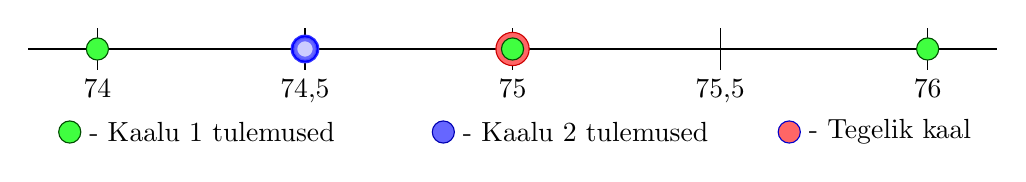
\begin{tikzpicture}
  \draw (0,0) -- (35em,0);
  \foreach \x/\xtext in {2.5/74,10/\text{74,5},17.5/75,25/\text{75,5},32.5/76}
  	\draw (\x em,0.75em) -- (\x em,-0.75em) node [anchor=north] {$\xtext$};
  \filldraw[fill=red!60,draw=red!80!black] (17.5em,0) circle [radius = 0.6em];
  \foreach \y in {2.5,17.5,32.5}
  	\filldraw[fill=green!75,draw=green!30!black] (\y em, 0) circle [radius = 0.4em];
  \filldraw[fill=blue!100,draw=blue!80] (10em,0) circle [radius = 0.5em];
  \filldraw[fill=blue!60,draw=blue!70] (10em,0) circle [radius = 0.4em];
  \filldraw[fill=blue!20,draw=blue!60] (10em,0) circle [radius = 0.3em];
  \filldraw[fill=green!75,draw=green!30!black] (1.5 em, -3em) circle [radius = 0.4em];
  \node[label=right: - Kaalu $1$ tulemused] at (1.5 em, -3em) {};
  \filldraw[fill=blue!60,draw=blue!70!black] (15em,-3em) circle [radius = 0.4em];
  \node[label=right: - Kaalu $2$ tulemused] at (15 em, -3em) {};
  \filldraw[fill=red!60,draw=blue!80!black] (27.5em,-3em) circle [radius = 0.4em];
  \node[label=right: - Tegelik kaal] at (27.5 em, -3em) {};
  
  
  
\end{tikzpicture}
}}
\caption{Kaalumiste tulemused kahe erineva kaaluga kolmel katsel}
\end{figure}

Kui mõista valiidsust kui testi keskmist tulemust, siis võime väita, et esimene kaal on väiksema reliaabluse aga suurema valiidsusega. Selline valiidsuse mõttestamine aga ei ole küsimustike modeleleerimise korral otstarbekas - katsete kordamine on enamasti keeruline ning väheste mõõtmistulemuste põhjal ei ole võimalik tegeliku väikese reliaablusega testi tulemust välja selgitada. 

Seega, meie vaadeldava olukorra - psühholoogiliste testide - korral on mingi valiidsuse taseme jaoks tarvilik tingimus mingi reliaabluse tase.    


\subsection{Sisemine järjepidevus}

Reliaabluse kui termini probleemiks on tema mitmetähenduslikus. Toome siinkohal ära ühe mõiste,  mida tihti samuti reliaablusena tuntakse.

Sisemine järjepidavus (\textit{internal consistency} on testi karrakteristik, mis iseloomustab testi erinevate k\"usimuste vastuste järjepidevust ehk seda, kui hästi on kooskõlas \"uhist  konstruktsiooni hindavad k\"usimused\cite[177] {Henson2001}. Piltlikult väljendudes, olgu meil järgnev k\"usimustik: 

\begin{figure}[H]

\colorbox{background_example}
	{\parbox
		{\textwidth}
			{
			\setlength{\unitlength}{1mm}
			\begin{picture}(148,55)
				\put(0,52){Käesolevat bakalaureusetööd on lihte lugeda.}
				\put(0,47){\line(1,0){14}}
				\put(8,41){Ei nõustu}
				\put(16,47){\circle{4}}
				\put(16,47){\circle*{2}}
				\put(18,47){\line(1,0){25}}
				\put(32,41){Ei nõustu osaliselt}
				\put(45,47){\circle{4}}
				\put(45,47){\circle*{2}}
				\put(47,47){\line(1,0){25}}
				\put(67,41){Nii ja Naa}
				\put(74,47){\circle{4}}
				\put(74,47){\circle*{2}}
				\put(76,47){\line(1,0){25}}
				\put(92,41){Nõustun osaliselt}
				\put(103,47){\circle{4}}
				\put(103,47){\circle*{2}}
				\put(105,47){\line(1,0){25}}
				\put(126,41){Nõustun}
				\put(132,47){\circle{4}}
				\put(132,47){\circle*{2}}
				\put(134,47){\vector(1,0){14}}
				\put(0,32){Mulle meeldib käesoleva bakalaureusetöö \"ulesehitus.}
				\put(0,27){\line(1,0){14}}
				\put(8,21){Ei nõustu}
				\put(16,27){\circle{4}}
				\put(16,27){\circle*{2}}
				\put(18,27){\line(1,0){25}}
				\put(32,21){Ei nõustu osaliselt}
				\put(45,27){\circle{4}}
				\put(45,27){\circle*{2}}
				\put(47,27){\line(1,0){25}}
				\put(67,21){Nii ja Naa}
				\put(74,27){\circle{4}}
				\put(74,27){\circle*{2}}
				\put(76,27){\line(1,0){25}}
				\put(92,21){Nõustun osaliselt}
				\put(103,27){\circle{4}}
				\put(103,27){\circle*{2}}
				\put(105,27){\line(1,0){25}}
				\put(126,21){Nõustun}
				\put(132,27){\circle{4}}
				\put(132,27){\circle*{2}}
				\put(134,27){\vector(1,0){14}}
				\put(0,12){Käesoleva bakalaureusetöö \"ulesehitus on loogiline.}
				\put(0,7){\line(1,0){14}}
				\put(8,1){Ei nõustu}
				\put(16,7){\circle{4}}
				\put(16,7){\circle*{2}}
				\put(18,7){\line(1,0){25}}
				\put(32,1){Ei nõustu osaliselt}
				\put(45,7){\circle{4}}
				\put(45,7){\circle*{2}}
				\put(47,7){\line(1,0){25}}
				\put(67,1){Nii ja Naa}
				\put(74,7){\circle{4}}
				\put(74,7){\circle*{2}}
				\put(76,7){\line(1,0){25}}
				\put(92,1){Nõustun osaliselt}
				\put(103,7){\circle{4}}
				\put(103,7){\circle*{2}}
				\put(105,7){\line(1,0){25}}
				\put(126,1){Nõustun}
				\put(132,7){\circle{4}}
				\put(132,7){\circle*{2}}
				\put(134,7){\vector(1,0){14}}
			\end{picture}
		}
		
	}
\caption{K\"usimustik bakalaureusetöö \"ulesehituse kohta }
\label{quiz_consistency}
\end{figure}

Siin on mõõdetavaks konstruktsiooniks käesoleva bakalaureusetöö \"ulesehitus ning sisemiseks reliaabluseks on vajalik kolmele näites toodud k\"usimusele antud vastuste kooskõla.

Selle karrakteristiku mõõtmiseks võimalik kasutada sisemise järjepidavuse teste. Segadust suurendab veelgi see, et üks nendest testidest leiab kasutamist ka meie poolt defineeritud reliaabluse hindamisel. Loodame, et nende kahe karakterisitku eristamine aitab lugejal käesolevas töös kergemini orienteeruda.

Märgime, et lisaks toodud kahele definitsioonile on ka teisi reliaabluse definitsioone \cite{Cronbach1947}, mis aga selle töö kontekstis ei tohiks segadust tekitada ning  mille äratoomist siin ei ole autor pidanud vajalikus.


\subsection{Probleemi püstitus}

Käesolevo tööga üritame pakkuda lahendusti kahele probleemile. Esimene nendest seisneb testi reliaabluse hindamises - kas on võimalik testi tulemuste põhjal hinnata selle testi reliaablust? 
Teine probleem lähtub esimesest - kui reliaabluse hindamine on võimalik, kas siis on võimalik kasutada saadud hinnangut Likerti skaala paremaks tõlgendamiseks intervallskaalana? Esimese probleemi rangeks mõtestamiseks vaatleme järgnevalt reliaablust ühe matemaatilise raamisitku - klassikalie testiteooria - kontekstis.

\pagebreak


\section{Reliaablus klassikalises testiteoorias}
Järgevas võtame aluseks Melvin Novicki klassikalise testiteooria \cite{Novick1966a}\cite{Lord1968} ja selle tõlgenduse Klaas Sijtsma poolt. \cite[109]{Sijtsma2009}

\subsection{Reliaabluse definitsioon}

\begin{meeldetuletus}
\begin{elementaarsyndmus}
\textit{Elementaarsündmuseks} nimetatakse juhusliku katse võimaliku tulemust.
\end{elementaarsyndmus}
\begin{toenaosus}
\textit{Tõenäosuseks} nimetatakse funktsiooni $P$, mis igale sündmusele $A \in 2^{\Omega}$, kus $\Omega$ on mingi juhusliku katse kõikvõimalikke elementaarsündmuste hulk, seab vastavusse arvu $P(A)$, nii et on täidetud järgmised nõuded:
\begin{enumerate}
\item $P(A) \geq 0, \forall A \in 2^{\Omega}$,
\item $P(\Omega) =1$, $P(\emptyset) = 0$,
\item Kui sündmused $A_1,A_2,...$ on teineteist välistavad, siis 
\begin{equation*}
 P\left( \bigcup \limits_{i=1}^{\infty} A_i \right) = \sum \limits_{i=1}^{\infty}P \left( A_i \right)
\end{equation*}.
\end{enumerate}
\end{toenaosus}
\begin{juhuslik_suurus}
\textit{Diskreetseks juhuslikus suuruseks} nimetatakse funktsiooni $X : \Omega \to \mathbb{R}$, mis võtab kas lõpliku või loenduva arvu erinevaid väärtusi $x_1,x_2,...(x_n)$.
\end{juhuslik_suurus}
\end{meeldetuletus}

Olgu meil mingi kogum $I$ testile vastajaid ning küsimustik, milles on $k$ k\"usimust, kus iga küsimus on $l$-pallisel Likerti skaalal. Nummerdame küsimused naturaalarvudega $1$ kuni $k$. On loomulik eeldada, et nii vastajate arv, küsimuste arv kui ka Likerti skaala suurus on lõplikud. Me võime vaadelda testi läbiviimist kui juhusliku katset ning kõike erinevaid võimalikke vastuste kombinatsioone küsimustikule kui elementaarsündmusi, tähistame saadud elementaarsündmuste hulga kui $\Omega$ ning elementaarsündmusi kui $\omega$. Eeldame ka tõenäosuste $P_i : 2^{\Omega} \to \mathbb{R}$ olemasolu, mida tõlgendame kui testi tulemuste esinemissagededust vastaja $i$ korral. 

\begin{figure}[H]
\begin{naide}
\begin{center}
\begin{tabular}{ | c | c c c |}
\hline
\diagbox{$\omega$}{Küsimus} & I & II & II \\
\hline
A & Nõustun osaliselt & Nii ja naa & Nõustun \\
B & Ei nõustu osaliselt & Nõustun & Nii ja naa \\
C & Ei nõustu & Nõustun osaliselt & Nii ja naa \\
\hline
\end{tabular}
\end{center}
\end{naide}
\caption{Näited elementaarsündmustest }
\end{figure}

Olgu $X_{i}^{j}$ hulgal $\Omega$ määratud juhuslik suurus, mille võimalike väärtusi vaatleme kui vastaja $i$ poolt k\"usimusele $j$ antud vastuse arvulist tõlgendust. On selge, et sellise tõlgenduse korral on juhusliku suuruse $X_{i}^{j}$ muutumispiirkond lõplik - selle hulga võimsus ei ole suurem kui $l$ ning järelikult on juhuslik suurus $X_{i}^{j}$ diskreetne. Defineerime vastaja $i$ testi tulemuse $X_{i}$ kui 

\begin{equation*}
X_{i} = \sum \limits_{j=1}^k X_{i}^{j} \text{.}
\end{equation*}


Paneme tähele, et $X_{i}$ on samuti diskreetne juhuslik suurus - tõepoolest, kuna tegemist on diskreetsete juhuslike suuruste summaga, siis on ta funktsioon hulgast $\Omega$ hulka $\mathbb{R}$. Lisaks, kuna kõikide liidetavate muutumispiirkond on tõkkestatud arvuga $l$ ning liidetavaid on $k$, siis ei saa funktsiooni muutumispiirkonna võimsus olla suurem kui $l^k$.


\begin{meeldetuletus}
\begin{jaotus} Disktreetse juhusliku suuruse $X$ \textit{jaotuseks} nimetatakse paaride komplekti $\left(x_i,p_i \right), i=1,2,...$, kus $x_i$ on juhusliku suuruse võimalik väärtus ning $p_i = P(\left\lbrace \omega | X(\omega) = x_i, \omega \in \Omega \right\rbrace)$. 
\end{jaotus}
\begin{keskvaartus}
Diskreetse juhusliku suuruse $X$, mille jaotuseks $K$ on paaride komplekt $k_i = \left(x_i,p_i \right), i=1,2,...$, \textit{keskväärtuseks} nimetatakse arvu
\begin{equation*}
 \epsilon X = \sum \limits_{\lbrace i | k_i \in K \rbrace} x_i p_i 
\end{equation*}
eeldusel, et see rida koondub absoluutselt.
\end{keskvaartus}
\begin{dispersioon}
Juhusliku suuruse $X$ \textit{dispersiooniks} nimetatakse arvu $DX = \epsilon \left[ (X-\epsilon X)^2 \right]$.
\end{dispersioon}
\end{meeldetuletus}

Triviaalse juhu vältimiseks eeldame edaspidi, et juhuslike suuruste $X_{i}$ dispersioonid on  nullist erinevad. Defineerime küsimustiku tegeliku tulemuse vastaja $i$ jaoks kui testi tulemuse keskväärtuse  ehk

\begin{equation*}
t_i = \epsilon  \left[ X_{i} \right] \text{.}\footnote{Tähistame keskväärtuse tähega $\epsilon$ kuna tavapärane tähistus $E$ leiab antud käsitluses teistsuguse rolli.}
\end{equation*}

Kuna juhusliku suuruse $X_{i}$ võimalike väärtuste arv on lõplik on ka tema keskväärtus $t_i$ lõplik. 


Tõlgendame vastaja $i$ testi tulemuse ja tegeliku tulemuse vahet mõõtmisveana, tähistame seda $E_i$. Seega $X_{i} = t_i + E_i$.


\begin{meeldetuletus}
\begin{keskvaartus_konstant}
\thlabel{keskvaartus_konstant}
Kui $X$ on diskreetne juhuslik suurus, jaotusega $K$, kus $K$ on paaride komplekt $k_i =(x_i,p_i), i=1,2,...$  ning $c$ on mingi konstant siis \linebreak $\epsilon(X+c) = \epsilon(X)+c$
\end{keskvaartus_konstant}
\begin{proof}
\begin{gather*}
\epsilon(X+c) = \sum \limits_{\lbrace i | k_i \in K \rbrace} (x_i + c) p_i  = \sum \limits_{\lbrace i | k_i \in K \rbrace} x_i p_i + \sum \limits_{\lbrace i | k_i \in K \rbrace} c p_i = \\ = \sum \limits_{\lbrace i | k_i \in K \rbrace} x_i p_i + c \sum \limits_{\lbrace i | k_i \in K \rbrace}  p_i  =   \sum \limits_{\lbrace i | k_i \in K \rbrace} x_i p_i + c  = \epsilon(X) + c
\end{gather*}
\end{proof}
\begin{dispersioon_konstant}
\thlabel{dispersioon_konstant}
Juhuslikule suurusele konstandi liitmine ei muuda dispersiooni : $D(X + c) = DX$
\end{dispersioon_konstant}
\begin{proof}
\begin{equation*}
D(X+c) = \epsilon[X+c - \epsilon(X+c)] \overset{\text{\thref{keskvaartus_konstant}}}{=} \epsilon[X+c - \epsilon(X) + c ] = \epsilon[X - \epsilon(X)] = DX
\end{equation*}
\end{proof}
\end{meeldetuletus}

Paneme tähele, et eelneva põhjal on vastaja $i$ mõõtmisvea keskväärtus võrdne nulliga. Tõepoolest, kuna tegeliku tulemuse definitsiooni põhjal $\epsilon \left[ X_{i} \right] = t_i$, siis saame mõõtmisvea definitsiooni arvesse võttes 

\begin{equation*}
 t_i = \epsilon \left[ X_{i} \right] = \epsilon \left[ t_i + E_i \right] \overset{\text{\thref{keskvaartus_konstant}}}{=} t_i + \epsilon \left[ E_i \right] \implies \epsilon \left[ E_i \right] = 0 \text{.}
\end{equation*}

Lisaks on lihtne märgata, et  $D \left[ X_{i} \right] = D \left[ E_i \right]$, sest 
\begin{equation*}
D \left[ X_{i} \right] = D \left[ E_i + t_i \right] \overset{\text{\thref{dispersioon_konstant}}}{=} D \left[ E_i \right] \text{.}
\end{equation*}  

Eelnevates definitsioonides keskendusime testi tulemuste mõtestamisele fikseeritud vastaja korral. Kuna reeglina mõtestatakse teste praktikas mingi vastajate kogumi raames, siis keskendume ka meie edaspidi sellele.

Vaatleme elementaarsündmustena hulga $I \times \Omega$ elemente ning eeldame, et eksisteerib tõenäosus
\begin{equation*}
P_p : 2^{I \times \Omega} \to \mathbb{R} \text{,}
\end{equation*} 
kus funktsiooni $P_p$ tõlgendame kui isiku $i \in I$ ja testi tulemuse $\omega \in \Omega$ koos esinemis sagedust.   


Paneme tähele, et sellel elemntaarsündmuste hulgal võime määrata diskreetse juhusliku suuruse $T$, nii et
\begin{equation*}
T\left((i, \omega)\right) = t_i, i \in I \text{.}
\end{equation*}

Seda juhuliku suurust tõlgendame kui küsimustiku tegelikku tulemust. Defineerime testi vaadeldava tulemuse kui diskreetse juhusliku suuruse $X$, nii et

\begin{equation*}
X \left (i, \omega) \right) = X_i (\omega) 
\end{equation*}
 
ja testi vea kui diskreetse juhusliku suuruse $E$, nii et

\begin{equation*}
E \left( (i, \omega) \right) = E_i (\omega) \text{.}
\end{equation*}

Paneme tähele, et kehtib $X = E + T$, tõepoolest olgu meil suvaline paar $\left(i, \omega \right) \in I \times \Omega$, siis 

\begin{equation*}
X \left( ( i, \omega ) \right) = X_i (\omega) \overset{def}{=}  t_i + E_i(\omega) = T \left( (i, \omega) \right) + E \left( ( i, \omega ) \right) \text{.} 
\end{equation*}

Eeldame edaspidises, et $X$ ei ole konstante juhuslik suurus - kui $X$ on konstante, siis .



\begin{meeldetuletus}
\begin{kovariatsioon}
Juhusliku suuruste $X$ ja $Y$ \textit{kovariatsiooniks} nimetatakse suurust
\begin{equation*}
cov(X,Y) = \epsilon \left[  \left( X - \epsilon X \right)\left(Y - \epsilon Y \right) \right]  \text{.}
\end{equation*}
\end{kovariatsioon}
\begin{korrelatsioon}
Juhusliku suuruste $X$ ja $Y$ \textit{korrelatsioonikordajaks} nimetatakse suurust 
\begin{equation*}
\rho (X,Y) = \frac{cov(X,Y)}{\sqrt{DX}\sqrt{DY}} 
\end{equation*}
\end{korrelatsioon}
\end{meeldetuletus}

Esitame nüüd meie poolt üles ehitatud mudeli omaduse, mis osutub väga kasulikus. Olgu meil kaks suvalist küsimustiku, mille vaadeldavad tulemused on vastavalt $X = T + E$ ja $X' = T' + E'$ , siis kehtib 
\begin{equation}
\label{eq:cov_zero}
cov(T,E') = 0 \text{,}
\end{equation} 
ehk mingi küsimustiku tegeliku tulemuse ja mingi küsimustiku mõõtmisvea vahel ei ole korrelatsiooni. See omadus muudab mudeli rakendamise palju lihtsamaks, kuna me ei pea eeldame, et meie poolt koostatud küsimustikul on selline omadus. Tõestus sellele omadusele kahjuks käesoleva töö raamidesse ei mahu, rangest tõestusest huvitatutele soovitame tutvuda Donald Zimmermani mudeli ülesehitusega \cite{Zimmerman1975}.

Paneme tähele, et kuna me ei seadunud mingeid kitsendusi testide $X$ ja $X'$ jaoks, siis ka $cov(T,E) = 0$.  

Küll aga peame me tegema järgneva eelduse - olgu meil kaks erinevat küsimustiku, mille mõõtmisvead on vastavalt $E$ ja $E'$ siis 
\begin{equation}
\label{eq:error_cov_0}
cov(E,E') = 0 \text{.}
\end{equation}

Tehtud eeldus tähendab seda, et mõõtmisvead ei tohi olla süstemaatilised. Näiteks, jagades küsimustiku pooleks ning vaadeldes mõlemat osa kui eraldi küsimustiku, siis teades esimese mõõtmisviga ei tohiks see meile midagi öelda teise osa mõõtmisvea kohta. Paneme tähele, et see eeldus on siimaani tehtutest praktikas kõige raskemini tagatav ning on potensiaalne ohukoht testiteooria kasutamisel mingi küsimustiku mõtestamisel. 


\begin{meeldetuletus}
\begin{summa_dispersioon}
\thlabel{summa_dispersioon}
Juhuslikke suuruste $X$ ja $Y$ puhul kehtib 
\begin{equation*}
D(X + Y) = D(X) + D(Y) + 2cov(X,Y)
\end{equation*} 
\begin{proof}
\begin{gather*}
D(X + Y) \overset{def}{=}\epsilon[X + Y - \epsilon(X + Y)]^2\overset{\text{$\epsilon$ lin.} }{=}  \epsilon [X - \epsilon X + Y + \epsilon Y]^2 = \\
 = \epsilon(X - \epsilon X)^2 + 2\epsilon (X - \epsilon X)(Y - \epsilon Y) + \epsilon (Y - \epsilon Y)^2   
 \overset{\text{cov  def}}{=}  \\   = D(X) + D(Y) + 2cov(X,Y)
\end{gather*}
\end{proof}
\end{summa_dispersioon}
\end{meeldetuletus}

Järgnevalt tutvume paralleelse küsimustiku mõistega. Kaks küsimustiku, mille vaadeldavad tulemused üle kõigi vastajate kogumi $I$ on $X = T + E$ ja $X' = T' + E'$ ning mille vaadeldavad tulemused vastaja $i \in I$ jaoks on $X_i = t_i + E_i$ ja $X_i' = t_i' + E_i'$ ,  on paralleelsed parajasti siis, kui kehtivad järgmised väited :
\begin{enumerate}
\item $t_i = t_i' ~ \forall i \in I  $,
\item $D \left[ E \right] = D \left[ E' \right] $. 
\end{enumerate}

Eelnevast järeldub lihtsalt, et  
\begin{equation}
\label{eq:true_scores_eq}
T = T' \text{.}
\end{equation} Tõepoolest, olgu $(i,\omega)$ suvaline paar hulgast $I \times \Omega$ , siis kehtib

\begin{equation*}
T((i, \omega) \overset{def}{=} t_i = t_i' = T'((i,\omega)) \text{.}
\end{equation*}

Paneme tähele, et kahe paraleelse küsimustiku $X$ ja $X'$ korral kehtib
\begin{equation}
\label{eq:par_dispersioon}
D[X] = D[X'] \text{,}
\end{equation}
kuna
\begin{gather*}
D[X] = D[T + E] \overset{\text{\thref{summa_dispersioon}}}{=}  D[T] + D[E] + 2cov(T,E) \overset{(\ref{eq:cov_zero})}{=} D[T] + D[E] = \\
= D[T'] + D[E'] = D[T'] + D[E'] + 2cov(T',E') = D[T' + E']  = D[X'] \text{.}
\end{gather*}

\begin{meeldetuletus}
\begin{summa_kovariatsioon}
\thlabel{summa_kovariatsioon}
Olgu meil juhuslikud suurused $X$, $Y$ ja $Z$. Siis 
\begin{equation*}
cov(X+Y,Z) = cov(X,Z) + cov(Y,Z)  \text{.}
\end{equation*}
\end{summa_kovariatsioon}
\begin{proof}
\begin{gather*}
cov(X+Y,Z) \overset{def}{=} \epsilon \left[(X+Y - \epsilon \left[ X + Y \right])(Z - \epsilon \left[ Z \right] ) \right] \overset{\text{$\epsilon$ lin.}}{=} \\
= \epsilon \left[ (X+Y - \epsilon \left[ X \right] +  \epsilon \left[ Y \right])(Z - \epsilon \left[ Z \right]  ) \right] = \\
= \epsilon \left[ ( \left( X - \epsilon \left[ X \right] \right) +  \left( Y -\epsilon \left[ Y \right]) \right) \left(Z - \epsilon \left[ Z \right] \right)  \right] = \\
=\epsilon [  \left( X - \epsilon \left[ X \right] \right) \left( Z - \epsilon \left[ Z \right] \right) +  
 \left( Y -\epsilon \left[ Y \right] \right) \left(Z - \epsilon \left[ Z \right] \right)  ] = \\
 =\epsilon \left[  \left( X - \epsilon \left[ X \right] \right) \left( Z - \epsilon \left[ Z \right] \right) \right] +   
\epsilon \left[  \left( Y -\epsilon \left[ Y \right] \right) \left(Z - \epsilon \left[ Z \right] \right) \right] +   \\ 
 = cov(X,Z) + cov(Y,Z)
\end{gather*}
\end{proof}
\end{meeldetuletus}


Paralleelse küsimustiku abil saame klassikalise testiteooria raames defineerida reliaabluse. Olgu meil kaks paralleelset küsimustiku, mille vaadeldavad tulemused \"ule vastajate kogumi $I$ on vastavalt $X = T + E$ ja $X' = T' + E'$. Testi, mille vaadeldav tulemus on $X$,  reliaablus \"ule vastajate kogumi $I$ on võrdne $X$ ja $X'$ korrelatsioonikordajaga, mida tähistame $\rho_{XX'}$, formaalselt

\begin{equation*}
\rho_{XX'} = corr \left( X,X' \right) \text{.}
\end{equation*} 


Eelneva põhjal saame näidata, et kehtib
\begin{equation}
\label{eq:corr_equals_var_over_var}
\begin{gathered}
\rho_{XX'} \overset{def}{=} \frac{cov(X,X')}{\sqrt{D \left[ X \right] D \left[ X' \right]}} \overset{(\ref{eq:par_dispersioon})}{=}   
\frac{cov(X,X')}{\sqrt{D \left[ X \right] D \left[ X \right]}} =  
\frac{cov(T+ E,T'+E')}{D \left[ X \right]} \overset{\text{\thref{summa_kovariatsioon}}}{=} \\ = 
 \frac{ cov(T,T') + cov(T,E') + cov(E,T') + cov(E,E')}{D \left[ X \right]} \overset{(\ref{eq:cov_zero})}{=} \\ 
 = \frac{ cov(T,T')  + cov(E,E')}{D \left[ X \right]} \overset{(\ref{eq:error_cov_0})}= \frac{ cov(T,T')}{D \left[ X \right]} \overset{(\ref{eq:true_scores_eq})}{=} \frac{cov(T,T)}{D \left[ X \right]} \overset{def}{=} \\
= \frac{\epsilon \left[\left( X - \epsilon \left[X \right] \right) \left( X - \epsilon \left[X \right] \right) \right]}{D \left[ X \right]} \overset{def}{=} \frac{D \left[T \right]}{D \left[ X \right]} \text{.}
\end{gathered}
\end{equation}

 Samuti märgime, et kuna $T = X - E$, siis kehtib
\begin{equation}
\label{eq:reliability}
\rho_{XX'} = \frac{D \left[ T \right]}{D \left[ X \right] } = \frac{D \left[ X - E \right]}{D \left[ X \right] } = \frac{D \left[X \right] - D \left[ E \right]}{D \left[ X \right]} = 1 - \frac{D \left[ E \right]}{D \left[ X \right]} \text{.}
\end{equation}

Paneme tähele, kuna $D[X] = D[T] + D[E]$, siis eelneva põhjal $\rho_{XX'} \in \left[0,1 \right]$.



Eelneva põhjal on selge, et väide  ``testi  reliaablus on suurem'' on samaväärne järgmise kolme väitega:
\begin{enumerate}
\item testi korrellatsioon paralleelse testiga on suurem,
\item testi tegeliku tulemuse dispersioon on suurem võrreldes testi vaadeldava tulemuse dispersiooniga,
\item testi mõõtmisvea dispersioon on väiksem võrreldes testi vaadeldava tulemuse dispersiooniga.
\end{enumerate}

Märgime, et klassikalise testiteooria raames defineeritud reliaablus sobib kokku eelmises peatükkis antud mitteformaalse definitsiooniga, kuna küsimustik on iseendaga paralleelne testiks võib lugeda ka sama testi uuesti läbiviimise sama vastajate kogumi peal. Paneme tähele, et tegemist on suhteliselt nõrku eeldusi vajava teooriaga, kõigi raskem on praktikas süstemaatiliste vigade puudumist. 

Kuna testi tegelik tulemus on suurus, mida me prakikas ei tea ning ka paralleelsete testide läbiviimine ei ole tihti võimalik on kasutusele on üritatud on võimalus testi reliaablust hinnata meie jaoks oluline. Järgnevalt vaatleme, kuidas seda teha.



\subsection{Vajalikud taustteadimesd reliaabluse hindamiseks}

Järgnev käsitlus tugineb Jacksoni ja Anguwamba 1977. aasta artiklile.\cite{Jackson1977}
Olgu meil küsimustik, milles on $k$ k\"usimust. Vaatleme seda klassikalise testi teooria raames ning olgu $X$ küsimustiku vaadeldav tulemus, $T$ küsimustiku tegelik tulemus ning $E$ küsimustiku mõõtmisviga. Vaatleme iga küsimust kui ühest küsimusest koosnevat alamküsimustiku ja tähistama fikseeritud k\"usimuse $ i \in \left\lbrace 1,2,\ldots,k \right\rbrace$ vaadeltavat tulemust kui $X_i$, tegeliku tulemust kui $T_i$ ning mõõtmisviga $E_i$. Seega $X = \sum \limits_{i=0}^{k} X_i$, $T = \sum \limits_{i=0}^{k} T_i$ ja $E = \sum \limits_{i=0}^{k} E_i$ . Paneme tähele, et kui eelnevas peatükkis tähistasime alaindeksiga küsimusele vastajat siis edaspidi tähistama sellega kindlat küsimust. 

Vaatleme testi k\"usimuste tulemuste ja mõõtmisvea vektoreid: $\left( X_1, X_2, X_3, \ldots, X_n \right)$, $\left( T_1, T_2, T_3, \ldots, T_n \right)$, $\left( E_1, E_2, E_3, \ldots, E_n \right)$. Tähistame nende vektorite kovariatsioonimaatriksid\footnote{Praktikas ei ole kovariatsioonimaatriksid meil teada, kuid meil on võimalik valimi põhjal saada hinnang vaadeldavate tulemuste kovariatsioonimaatriksile }, vastavalt $\Sigma_X, \Sigma_T, \Sigma_E$. Seega, 
\small
\begin{equation*}
\Sigma_X = 
\begin{pmatrix}
cov \left(X_1,X_1 \right) && cov\left( X_1,X_2 \right) && cov \left( X_1,X_3 \right) && \cdots && cov \left( X_1,X_k \right) \\
cov \left(X_2, X_1 \right) && cov \left(X_2, X_2 \right) && cov \left(X_2, X_3 \right) && \cdots && cov \left(X_2, X_n \right) \\
cov \left(X_3, X_1 \right) && cov \left(X_3, X_2 \right) && cov \left(X_3, X_3 \right) && \cdots && cov \left(X_n, X_n \right) \\
\vdots && \vdots && \vdots && \ddots && \vdots \\
cov \left(X_n, X_1 \right) && cov \left(X_n, X_2 \right) && cov \left(X_n, X_3 \right) && \cdots && cov \left(X_n, X_n \right) \\
\end{pmatrix}.
\end{equation*}
\normalsize

Eelnevalt läbiviidud arutelu (vt. (\ref{eq:corr_equals_var_over_var})) põhjal teame, et $cov(X_i,X_j) = cov(T_i,T_j) + cov(E_j,E_j)$. Seega, 

\begin{equation}
\label{eq:sigma_x_=_sigma_t_+_sigma_e}
\Sigma_X = \Sigma_T + \Sigma_E \text{.}
\end{equation}

Lisaks kehtib eelduse (\ref{eq:error_cov_0}) põhjal saame, et et juhul kui $i \neq j$, siis $cov \left( E_i, E_j \right) = 0$.
Sellest tulenevalt kehtib

\small
\begin{equation}
\label{eq:sigma_E}
\Sigma_E = 
\begin{pmatrix}
cov \left(E_1,E_1 \right) && 0 && 0 && \cdots && 0 \\
0 && cov \left(E_2, E_2 \right) && 0 && \cdots && 0 \\
0 && 0 && cov \left(E_3, E_3 \right) && \cdots && 0 \\
\vdots && \vdots && \vdots && \ddots && \vdots \\
0 && 0 &&  0 && \cdots && cov \left(E_n, E_n \right) \\
\end{pmatrix}.
\end{equation}
\normalsize

Tähistame edaspidi maatriksi $\Sigma_X$ elemente  $x_{ij}$, maatriksi $\Sigma_T$ elemente $x_{ij}$ ning maatriksi $\Sigma_E$ peadiagonaali elemente $\theta_i$. Seega, kui $i \neq j$, siis $t_{ij} = x_{ij}$ ning $t_{ii} = x_{ii} - \theta_i$.

Tuletame meelde, et eelmises peatükkis veendusime (\ref{eq:reliability}), et testi reliaablus võrdub avaldisega $1 - \frac{D \left[ E \right]}{D \left[ X \right]}$. 

Veendume, et juhuslike suuruste summa summa dispersioon võrdub liidetavate kovariatsioonimaatriksi elementide summaga ehk kui $X = \sum \limits_{i=1}^k$  ja $\Sigma_X$ on vektori $(X_1,X_2,\ldots,X_K)$ kovariatsioonimaatriks siis
\begin{equation*}
D[X] = \sum \limits_{i=1}^k \sum \limits_{j=1}^k {\Sigma_X}_{ij} \text{.}
\end{equation*}

Eelnevas veendumiseks paneme tähele, et 
\begin{gather*}
D[X] =  D[X_1 + X_2 + \ldots + X_k] \overset{\text{\thref{summa_dispersioon}}}{=} \\ = D[X_1] + D[X_2 + X_3 + \ldots + X_k]   + 2cov(X_1,X_2 + X_3 \ldots + X_k)\overset{\text{\thref{summa_kovariatsioon}}}{=} \\
= D[X_1] +  D[X_2 + X_3 + \ldots + X_k]  + \\
+ 2[ cov(X_1,X_2) + cov(X_1,X_3) + \ldots + cov(X_1,X_k)] \text{.}
\end{gather*}

Näeme, et tegemist on rekkurentse võrrandiga. Arvestades, et $cov(X,X) = D[X]$ (vt.(\ref{eq:corr_equals_var_over_var})), näeme, et igale liidetavale eelnevas summas vastab mingite kovariatsioonimaatriksite elementide summa, kusjuures kõik kovariatsioonimaatriksi elemendid kuuluvad täpselt ühte nendest summadest. Kovariatsiooni maatriksi jagunemist illustreerib järgnev tabel, kus sinisega on tähistatud $D[X_1]$, punasega liidetavad, mille summa on võrdne arvuga $2[ cov(X_1,X_2) + cov(X_1,X_3) + \ldots + cov(X_1,X_k)]$ ja rohelisega liikmed, mille summast moodustub $D[X_1 + X_2 + \ldots + X_k]$.


\begin{figure}[H]
\centering
{\renewcommand*{\arraystretch}{1.5} \begin{tabular}{|c  c c  c  c|}
\hline
\cellcolor{blue!20}$cov(X_1,X_1)$ & {\cellcolor{red!20}$cov(X_1,X_2)$} & \cellcolor{red!20}$cov(X_1,X_3)$ & \cellcolor{red!20}$\hdots$ & \cellcolor{red!20}$cov(X_1,X_k)$  \\
\cellcolor{red!20}$cov(X_2,X_1)$ & \cellcolor{green!50!black!50}$cov(X_2,X_2)$ & \cellcolor{green!50!black!50}$cov(X_2,X_3)$ & \cellcolor{green!50!black!50}$\hdots$ & \cellcolor{green!50!black!50}$cov(X_1,X_k)$ \\
\cellcolor{red!20}$cov(X_3,X_1)$ & \cellcolor{green!50!black!50}$cov(X_3,X_2)$ & \cellcolor{green!50!black!50}$cov(X_3,X_3)$ & \cellcolor{green!50!black!50}$\hdots$ & \cellcolor{green!50!black!50}$cov(X_3,X_k)$ \\
\cellcolor{red!20}$\vdots$ & \cellcolor{green!50!black!50}$\vdots$ & \cellcolor{green!50!black!50}$\vdots$ & \cellcolor{green!50!black!50}$\ddots$ & \cellcolor{green!50!black!50}$\vdots$ \\
\cellcolor{red!20}$cov(X_k,X_1)$ & \cellcolor{green!50!black!50}$cov(X_k,X_2)$ & \cellcolor{green!50!black!50}$cov(X_k,X_3)$ & \cellcolor{green!50!black!50}$\hdots$ & \cellcolor{green!50!black!50}$cov(X_k,X_k)$ \\
\hline
\end{tabular}}
\end{figure}

Lisaks on sellel rekurentses võrandil on lihtne baasjuht, selleks on olukord, kus summa koosneb ainult ühest liidetavast. 

Arvestades maatriksi \ref{eq:sigma_E} ehitust, saame võrduse 

\begin{equation}
\label{eq:reliability_cov}
1 - \frac{D \left[ E \right]}{D \left[ X \right]} = 1 - \frac{\sum_i \theta_i }{\sum_i \sum_j x_{ij}}.
\end{equation}

\begin{meeldetuletus}
\begin{mittenegatiivselt_maaratud} Maatriks $C \in Mat_k(\mathbb{R})$ on \textit{mittenegatiivselt määratud} kui iga maatriksi $v \in Mat_{k,1}(\mathbb{R})$ korral $v^T C v \geq 0$.
\end{mittenegatiivselt_maaratud}
\end{meeldetuletus}

Veendume järgnevalt, et iga kovariatsioonimaatriks ning järelikult ka $\Sigma_X, \Sigma_T$ ja $ \Sigma_E$ on mittenegatiivselt määratud. 

\begin{meeldetuletus}
\begin{konstant_kovariatsioon}
\thlabel{konstant_kovariatsioon}
Kui $X$ ja $Y$ on juhuslikud suurused ja $\alpha \in \mathbb{R}$, siis
\begin{equation*}
cov(X,\alpha Y) = \alpha cov(X,Y)
\end{equation*}
\end{konstant_kovariatsioon}
\begin{proof}
\begin{gather*}
cov(X,\alpha Y) = \epsilon \left[ \left( X - \epsilon \left[ X \right] \right) \left( \alpha Y - \epsilon \left[ \alpha Y \right] \right) \right] \overset{\text{$\epsilon$ lin.}}{=}  \\ = \epsilon \left[ \left( X - \epsilon \left[ X \right] \right) \left( \alpha Y - \alpha \epsilon \left[ Y \right] \right) \right] = 
 \epsilon \left[\alpha \left( X - \epsilon \left[ X \right] \right) \left( Y -  \epsilon \left[ Y \right] \right) \right] = \\
 =  \alpha \epsilon \left[ \left( X - \epsilon \left[ X \right] \right) \left( Y -  \epsilon \left[ Y \right] \right) \right] = \alpha cov(X,Y)
\end{gather*}
\end{proof}
\end{meeldetuletus}

Olgu meil suvaliste juhuslike suuruste vektor $X_1,X_2,\ldots,X_n$ , kun $n \in \mathbb{N}$ ja olgu $\Sigma_X$ selle vektori kovariatsioonimaatriks. Olgu meil suvaline $k$-vektor $v = (v_1,v_2,\ldots,v_n)$. Konstrueerime uue juhuslike suuruste vektori ($X_1',X_2',\ldots,X_n')$, kusjuures $X_i' = v_i X_i$ ning olgu $\Sigma_X'$ selle vektori kovariatsioonimaatriks. Vaatleme juhusliku suurust $X' = \sum \limits_{i=1}^n X_i'$. Kuna eelneva põhjal $D[X'] = \sum \limits_{i=1}^n \sum \limits_{j=1}^n {\Sigma_X'}_{ij} $ ja definitsiooni põhjal $D[X'] \geq 0$, siis $\sum \limits_{i=1}^n \sum \limits_{j=1}^n {\Sigma_X}_{ij} \geq 0$. Kuna $\Sigma_X'$ on kovariatsioonimaatriks siis,
\begin{equation}
\label{eq:kov_maatriksi_summa}
\sum \limits_{i=1}^n \sum \limits_{j=1}^n {\Sigma_X'}_{ij} = \sum \limits_{i=1}^n \sum \limits_{j=1}^n cov(v_iX_i,v_jX_j) \overset{\text{\thref{konstant_kovariatsioon}}}{=} \sum \limits_{i=1}^n \sum \limits_{j=1}^n v_i v_j cov(X_i,X_j) \text{.}
\end{equation}

Paneme tähele, et 

\begin{gather*}
v^T \Sigma_X v = \\
= \begin{pmatrix}
v_1 cov(X_1,X_1) + v_2 cov(X_1,X_2) + \hdots v_n cov(X_1,X_n) \\
v_1 cov(X_2,X_1) + v_2 cov(X_2,X_2) + \hdots v_n cov(X_2,X_n) \\
\vdots \\
v_1 cov(X_k,X_1) + v_2 cov(X_k,X_2) + \ldots v_n cov(X_n,X_n) \\
\end{pmatrix} v = \\  \sum \limits_{i=1}^n \sum \limits_{j=1}^n v_i v_j cov(X_i,X_j)  \overset{(\ref{eq:kov_maatriksi_summa})}{=} \sum \limits_{i=1}^n \sum \limits_{j=1}^n {\Sigma_X'}_{ij} = D[X']
\end{gather*}
Seega $v^T \Sigma_X v \geq 0$ ning kuna $v$ oli valitud suvaliselt siis on $\Sigma_X$ mittenegatiivselt määratud. Kuna $n$ ja $X_1,X_2,\ldots X_n$ olid valitud suvaliselt, siis on iga kovariatsioonimaatriks mittenegatiivselt määratud. 

Sellega oleme andund reliaablusele matemaatilise definitsiooni ning mõtestanud lahti vajaminevad taustteadmised reliaabluse hindamiseks. Järgnevalt tuletame mõned alumised tõkked reliaablusele.   

  
 {\color{red}- - - SIIA MAANI REFAKTOREERITUD! EDASI OMAL VASTUTUSEL! - - - -} 

\section{Alumised tõkked reliaablusele}

Järgnevalt vaatleme viite alumist tõket reliaablusele, millest neli - $\lambda_1,\lambda_2,\lambda_3,\lambda_4$; pakkus aastal 1945 välja Louis Guttman \cite{Guttman1945}. Viienda vaadeldava tõkke pakkusid välja Jackson ja Anguwamba oma 1977 aasta artiklis \cite{Jackson1977}. Kõik tõkked tuletame tuginedes Jacksoni ja Anguwamba artiklile.

\subsection{Alumine tõke $\lambda_1$}

Vaatleme kovariatsioonimaatriksit $\Sigma_T \in Mat(k)$. Leidugu maatriksi peadiagonaalil element, mis on negatiivne. Olgu selle elemendi indeks $i$. Olgu $v$ vektor, millel on $k$ elementi, kusjuures 
\begin{equation}
v_j =
\begin{cases}
1, j = 1 \\
0, j \neq 1
\end{cases} 
\end{equation} 

Paneme tähele, et n\"u\"ud $v^T \Sigma_T v = t_i < 0$. Seega ei ole maatriks enam positiivselt määratud ja ei saa olla kovariatsioonimaatriks.

Seega iga $i$ peab kehtima $t_i \geq 0$ ning seega $\theta_i < x_i$ {\color{cyan}Kas on okay peadiagonaalile viidata \"uhe indeksiga? Peaks kuhugi kirjutama või minema \"ule kahe indeksi peale ? }.

Seega ka $\sum \nolimits_i \theta \leq \sum \nolimits x_i$. Seega saame \ref{eq:reliability_cov} põhjal kirja panna reliaabluse alumise tõkku, mida tähistame kui $\lambda_1$,
\begin{equation}
\lambda_1 = 1 - \frac{\sum_i x_i}{\sum_i \sum_j x_{ij}} \leq  1 - \frac{\sum_i \theta_i}{\sum_i \sum_j x_{ij}} =  1 - \frac{D \left[ E \right]}{D \left[ X \right]}.
\end{equation} 

\subsection{Alumine tõke $\lambda_2$}

Enne järgmise alumise tõke tuletamist, veendume et kehtivad kaks abitulemust.

Olgu meil mitte-negatiivselt määratud s\"ummeetriline maatriks $C, C \in Mat(n)$. Näitame, et sellisel juhul kehtib väide, et iga $i,j$ korral
\begin{equation*}
c_{i}c_{j} \geq c_{ij}^2 
\end{equation*}

Valime suvaliselt $i$ ja $j$, nii et $i \neq j, i,j \leq n$ ning $\alpha \in \mathbb{R}$. Olgu meil $n$-vektor $v$, kus
\begin{equation*}
v_k =
\begin{cases}
1, k=i \\
\alpha, k=j \\
0, k \not \in \lbrace i, j \rbrace \\
\end{cases}
\end{equation*}.

Kuna $C$ on eelduste kohaselt mitte-negatiivlet määratud, siis peab kehtima 
\begin{equation}
\label{eq:sd-toestus-maatriks-korrutis}
0 \leq v^{T}Cv = 
\begin{pmatrix}
\mathbf{0}^T & 1 & \mathbf{0'}^T & \alpha & \mathbf{0''}^T
\end{pmatrix}
\begin{pmatrix}
c_{11} && \cdots && c_{1n} \\
\vdots && \ddots && \vdots \\
c_{n1} && \cdots && c_{nn}  
\end{pmatrix}
\begin{pmatrix}
\mathbf{0}^T & 1 & \mathbf{0'}^T & \alpha & \mathbf{0''}^T
\end{pmatrix},
\end{equation}

kus $\mathbf{0},\mathbf{0'},\mathbf{0''}$ on null vektorit pikkustega vastavlt $i-1,j-i-1, n -j$.



Arvutame avaldise \ref{eq:sd-toestus-maatriks-korrutis} väärtuse:

\begin{equation*}
\begin{split}
v^{T}Cv =
\begin{pmatrix}
\mathbf{0}^T & 1 & \mathbf{0'}^T & \alpha & \mathbf{0''}^T
\end{pmatrix}
\begin{pmatrix}
c_{11} && \cdots && c_{1n} \\
\vdots && \ddots && \vdots \\
c_{n1} && \cdots && c_{nn}  
\end{pmatrix}
\begin{pmatrix}
\mathbf{0}^T & 1 & \mathbf{0'}^T & \alpha & \mathbf{0''}^T
\end{pmatrix} = \\
= \begin{pmatrix}
\mathbf{0}^T & 1 & \mathbf{0'}^T & \alpha & \mathbf{0''}^T
\end{pmatrix}
\begin{pmatrix}
c_{1i} + \alpha c_{1j} \\
\vdots \\
a_{ni} + \alpha c_{nj} 
\end{pmatrix}
= c_{i} + \alpha c_{ij} + \alpha c_{ji} + \alpha^2 c_{j} = c_i + 2 \alpha c_{ij} + \alpha^2 c_{j}.
\end{split}
\end{equation*}


See, et saadud ruutvõrratus on rahuldatud on samaväärne sellega, et 
\begin{equation*}
c_{ij}^2 - c_{i}c_{j} \leq 0,
\end{equation*}
milles me soovisimegi veenduda. Eelneva arutelu pärineb Ivar Tammeraidi raamatust \cite{Tammeraid1999}.  

Paneme n\"u\"ud tähele, et kehtib järgvev algebraline samasus:  
\begin{equation*}
\left( \sum_i x_i \right)^2 =   \sum_i x_i^2 + \underset{i \neq j}{\sum_i \sum_j} x_i x_j
\end{equation*}

Kuna eelnev kehtib, siis kehtib ka 

\begin{equation*}
2 \left( n-1 \right) \left( \sum_i x_i \right)^2 =  2 \left( n-1 \right) \sum_i x_i^2 + 2 \left( n-1 \right) \underset{i \neq j}{\sum_i \sum_j} x_i x_j
\end{equation*}

Liidetavad teistmoodi grupeerides saame, et
\begin{equation*}
\begin{gathered}
2 \left( n-1 \right) \sum_i x_i^2 + 2 \left( n-1 \right) \underset{i \neq j}{\sum_i \sum_j} x_i x_j = \\
= \left( x_{1}^2 - 2 x_1 x_2 + x_{2}^2 \right) + \left( x_{1}^2 - 2 x_1 x_3 + x_{3}^2 \right) + \cdots + \left( x_{2}^2 - 2 x_1 x_2 + x_{1}^2 \right) + \cdots + 2n \underset{i \neq j}{\sum_i \sum_j} x_i x_j = \\
= \underset{i \neq j}{\sum_i \sum_j} (x_i -  x_j)^2 + 2n \underset{i \neq j}{\sum_i \sum_j} x_i x_j
\end{gathered}
\end{equation*}

Vaatleme jällegi kovariatsiooni maatriksit $\Sigma_E$. Märkame, et kehtib järgnev:

\begin{equation*}
tr \left( \Sigma_E \right) = \sum_i \theta_i = \sum_i x_i - \sum_i t_i 
\end{equation*}.

Eelnevalt käsitletud algebralise samasuse põhjal on lihtne veenduda, et kehtib

\begin{equation*}
\sum_i t_i = \sqrt{\frac{\underset{i \neq j}{\sum_i \sum_j} (t_i -  t_j)^2 + 2n \left( \underset{i \neq j}{\sum_i \sum_j} t_i t_j \right) }{2 \left( n -1 \right)}} \geq \sqrt{\frac{ n \left( \underset{i \neq j}{\sum_i \sum_j} t_i t_j \right) }{\left( n -1 \right)}}
\end{equation*}

Arvestades, et kovariatsioonimaatriks on mitte-negatiivselt määratud ning seda, et kui $i \neq j$ siis $t_{ij} = x_{ij}$ , saame eelnevalt tõestatud abitulemuse põhjal väita, et

\begin{equation*}
\sum_i t_i  \geq \sqrt{\frac{ n \left( \underset{i \neq j}{\sum_i \sum_j} t_i t_j \right) }{\left( n -1 \right)}} \geq \sqrt{\frac{ n \left( \underset{i \neq j}{\sum_i \sum_j} x_{ij}^2 \right) }{\left( n -1 \right)}}
\end{equation*} 

Selle taustal saame defineerida alumise tõkke reliaablusele, mida tähistame $\lambda_2$:

\begin{equation*}
\lambda_2 = 1 - \frac{\sum_i x_i - \sqrt{\frac{ n \left( \underset{i \neq j}{\sum_i \sum_j} x_{ij}^2 \right) }{\left( n -1 \right)}}}{\sum_i \sum_j x_{ij}} \leq 1 - \frac{\sum_i x_i - \sum_i t_i}{\sum_i \sum_j x_{ij}} =   1 - \frac{\sum_i \theta_i}{\sum_i \sum_j x_{ij}} =  1 - \frac{D \left[ E \right]}{D \left[ X \right]} \text{.}
\end{equation*}


\subsection{Alumine tõke $\lambda3$}

Vaatleme jällegi kovariatsioonimaatriksit $\Sigma_T$. Olgu meil $n$-vektor $v$, mille elment kohal $i$ on $1$ ja element kohal $j$ on $-1$. Kuna kovariatsioonimaatriks peab olema mittenegatiivselt määratud siis peab kehtima

\begin{equation*}
\label{eq:psd 1 -1 vector}
0 \leq v^T \Sigma_T v = v^T 
\begin{pmatrix}
t_{1i} - t_{1j} \\
t_{2i} - t_{2j} \\
\vdots \\
t_{ni} - t{nj} \\
\end{pmatrix}
= t_{i} + t_{j} - 2 t_{ij} \text{,}
\end{equation*}

võttes arvesse seda, et kui $i \neq j$, siis $x_{ij} = t_{ij}$ saame, et $t_i + t_j \geq 2 x_{ij}$. 

Teame, et võimalusi valida $i$ ja $j$ nii, et $i \neq j$ on $n \left( n -1 \right)$. Summeerides kõik võimalikud võrratused saame, et
\begin{equation*}
2 \left( n - 1 \right) \sum_i t_i \geq 2  \underset{i \neq j}{\sum_i \sum_j} x_{ij},
\end{equation*}
mis on samaväärne sellega, et

\begin{equation*}
\sum_i t_i \geq  \frac{1}{n - 1} \underset{i \neq j}{\sum_i \sum_j} x_{ij}.
\end{equation*}


Niisiis, oleme saanud järgmise alumise tõkke reliaablusele, 
\begin{equation*}
\lambda_3 = 1 - \frac{\sum_i x_i - \frac{1}{n-1}{\underset{i \neq j}{\sum_i \sum_j} x_{ij}}}{\sum_i \sum_j x_{ij}} \leq  1 - \frac{\sum_i x_i - \sum_i t_i}{\sum_i \sum_j x_{ij}} =   1 - \frac{\sum_i \theta_i}{\sum_i \sum_j x_{ij}} =  1 - \frac{D \left[ E \right]}{D \left[ X \right]} \text{.}
\end{equation*}

Tõkke lihtsustamisel algebraliste samaväärsustega saame, et

\begin{equation*}
\begin{gathered}
\lambda_3 = 1 - \frac{\sum_i x_i - \frac{1}{n-1}{\underset{i \neq j}{\sum_i \sum_j} x_{ij}}}{\sum_i \sum_j x_{ij}} =  \frac{\sum_i \sum_j x_{ij} -  \sum_i x_i + \frac{1}{n-1}{\underset{i \neq j}{\sum_i \sum_j} x_{ij}}  }{\sum_i \sum_j x_{ij}} = \\
= \frac{{\underset{i \neq j}{\sum_i \sum_j} x_{ij}} + \frac{1}{n-1}{\underset{i \neq j}{\sum_i \sum_j} x_{ij}}}{\sum_i \sum_j x_{ij}} = \frac{n}{n-1} \left( \frac{\underset{i \neq j}{\sum_i \sum_j} x_{ij}}{\sum_i \sum_j x_{ij}} \right) = \frac{n}{n-1} \left(1 - \frac{\sum_i x_{i}}{\sum_i \sum_j x_{ij}} \right).
\end{gathered}
\end{equation*}

Tuletades meelde tõkke $\lambda_1$ definitsiooni on ilmne, et
\begin{equation}
\label{eq:lambda_3_from_lambda_1}
\lambda_3 = \frac{n\ \lambda_1}{n-1}.
\end{equation}
 

 
\subsection{Alumine tõke $\lambda_4$}

Nagu eelmise kahe tõkku puhul, vaatleme kovariatsioonimaatriksit $\Sigma_T$. Olgu meil vektor $v$ selline, et $\lvert {v_i} \rvert = 1$ iga $i \leq n, i \in \mathbb{N}$ korral.    
Teame, et kehtib
\begin{equation*}
0 \leq v^{T} \Sigma_T v,
\end{equation*}
seega arvestades kovariatsioonimaatriksi $\Sigma_E$ omadusi saame võrduse \eqref{eq:sigma_x_=_sigma_t_+_sigma_e} põhjal 

\begin{equation*}
\sum_i \theta_i = \sum_i v_{i}^{2} \theta_i = v^{T} \Sigma_E v \leq v^{T} \Sigma_X v.
\end{equation*}

Seega, iga võimaliku $v$ korral saame alumise tõkke reliaablusele. Tõepoolest, \eqref{eq:reliability_cov} põhjal iga $v$ korral,  
\begin{equation*}
1 - \frac{v^T \Sigma_X v}{\sum_i \sum_j x_{ij}} \leq 1 - \frac{\sum_i \theta_i}{\sum_i \sum_j x_{ij}} = 1 - \frac{D \left[ E \right]}{ D \left[X \right]  }
\end{equation*} 
Defineerime alumise tõkke $\lambda_4$ kui maksimumi kõikidest sellistest tõkketest, seega

\begin{equation*}
\lambda_4  = \underset{v}{max} \left( 1 - \frac{v^{T} \Sigma_X v}{\sum_i \sum_j x_{ij}} \right).
\end{equation*}


\subsection{Alumine tõke $glb$}

Me teame, et kehtib \eqref{eq:sigma_x_=_sigma_t_+_sigma_e} ning teame, et $\Sigma_X$, $\Sigma_T$ ja $\Sigma_E$ on kovariatsioonimaatriksid, seega ka mitte-negatiivselt määratud.

Paneme tähele, et tänu $\Sigma_E$ struktuurile on tema mittenegatiivsus samaväärne sellega, et $0 \leq \theta_i$ iga $i$ korral {\color{cyan} Tõestus? Iseenesest väga lihtne}. 

\"Uritame n\"u\"ud  leida vea suurimat võimaliku dispersiooni, mis on \eqref{eq:reliability} põhjal samaväärne summaga $\sum_i \theta_i$, arvestades eelnevalt kirjeldatud piiranguid. Saame selle panna kirja järgneva optimiseerimis\"ulesandena:
\begin{equation}
\begin{gathered}
max \sum_i \theta_i \\
\theta_i > 0 \\
\Sigma_X = \Sigma_T + \Sigma_E \\
\Sigma_T \succeq 0, \\
\end{gathered} 
\end{equation} 

kus kirjapilt $\Sigma_T \succeq 0$ tähistab tingimust "$\Sigma_T$ on mittenegatiivselt määratud". 

Olgu $z$ eelneva optimiseerimis\"ulesande lahend mingi fikseeritud vaadelud tulemuste kovariatsioonimaatrikis $\Sigma_X$ korral. Tähistame tähekombinatsiooniga $glb$, mis tuleneb fraasist \textit{greatest lower bound}, $z$ abil saadud alumise tõkku reliaablusele ehk

\begin{equation*}
glb = 1 - \frac{z}{\sum_i \sum_j x_{ij}}.
\end{equation*}  

Panemet tähele, et kuna $z$ on maksimaalne vea dispersioon fikseeritud $\Sigma_X$ korral, siis on alumine tõke $glb$ minimaalne võimalik reliaablus. Siit aga saame, et iga teine reliaabluse alumine tõke peab olema väiksem võrdne tõkega $glb$. Seega on $glb$ suurim võimalik alumine tõke. 






\subsection{Cronbachi alfa}

Cronbachi alfa on levinud sisemist reliaablust iseloomustav näitaja, mis on defineeritud järgnevalt:

\begin{equation}
(\frac{k}{k-1})( 1 - \frac{\sum \sigma_i^2}{\sigma_t^2})
\end{equation}

kus $k$ tähistab k\"usimuste arvu, $\sigma_i$ on standardviga \"uhe k\"usimuse piires ja $\sigma_t$ on standardviga \"ule testi kogutulemuste.\cite[396]{Cronbach2004}

{\color{cyan} Siia selgitav näidis tabel/joonis vajalik?}


\paragraph{Miks ma taandan selles töös sisemise järjekindluse mõõtmise Cronbachi alfale?}\mbox{}\\*

Kuna Cronbach'i alfal on mitmeid puuduseid, millest mõningad on toodud ära David Streineri artiklis \cite[101-102]{Streiner2010}, ning isegi mõõdiku autor Lee Cronbach soovitab oma 1951. aastal välja töötatud mõõdiku asemel kasutatada alternatiivseid mõõdikuid \cite{Cronbach2004}, on oluline vastata alapealkirjas p\"ustitatud k\"usimusele. Kaks peamist põhjust on järgnevad:
\begin{enumerate}[I]
\item Cronbachi alfa on hetkel kõige kasutatavam mõõdik sisemise reliaabluse mõõtmiseks ps\"uhho-meetriliste testide juures. Seetõttu on väljapakutud meetod testide tulemuste anal\"u\"usijatele tuttav ning seega loodetavasti lihtsamini kasutatav.
\item Cronbachi alfa leidmine on arvutuslikult k\"ullaltki lihtne. Kuna käesoleva töö peamine eesmärk on selgitada, kas väljapakutud lähenemine on mõistlik, siis ei ole parematest mõõdikutest potentsiaalselt saadav kasu piisavalt suur, et tasa teha \"ulesande lahendamise raskemaks muutumist. Juhul, kui töö tulemus on aga positiivne,  tuleks uurida ka teiste mõõdikute võimalikku kasutamist.

\end{enumerate}










\section{\"Ulesande p\"ustitus}

Selle töö raames loodame välja pakkuda viisi, kuidas paigutada intervallskaalal erinevaid vastuseid Likerti skaalalt. Eesmärk on leida parem paigutus kui vaikimisi meetod, kus eeldatakse, et erinevate hinnagute vahekaugused on samad. Vaatleme kahte näidet:


\begin{figure}[H]


\colorbox{background_example}
	{\parbox
		{\textwidth}
			{
			\setlength{\unitlength}{1mm}
			\begin{picture}(148,15)
				\put(0,12){Käesoleva bakalaureusetöö \"ulesehitus on loogiline.}
				\put(0,7){\line(1,0){14}}
				\put(8,1){Ei nõustu}
				\put(16,7){\circle{4}}
				\put(16,7){\circle*{2}}
				\put(18,7){\line(1,0){25}}
				\put(32,1){Ei nõustu osaliselt}
				\put(45,7){\circle{4}}
				\put(45,7){\circle*{2}}
				\put(47,7){\line(1,0){25}}
				\put(67,1){Nii ja Naa}
				\put(74,7){\circle{4}}
				\put(74,7){\circle*{2}}
				\put(76,7){\line(1,0){25}}
				\put(92,1){Nõustun osaliselt}
				\put(103,7){\circle{4}}
				\put(103,7){\circle*{2}}
				\put(105,7){\line(1,0){25}}
				\put(126,1){Nõustun}
				\put(132,7){\circle{4}}
				\put(132,7){\circle*{2}}
				\put(134,7){\vector(1,0){14}}
			\end{picture}
		}
		
	}
\caption{Näide, kuidas hinnangud skaalal hetkel vaikimisi meetodit kasutades paigutuvad}
\label{quiz}
\end{figure}

\begin{figure}[H]


	\colorbox{background_example}
	{\parbox
		{\textwidth}
			{
			\setlength{\unitlength}{1mm}
			\begin{picture}(148,15)
				\put(0,12){Käesoleva bakalaureusetöö \"ulesehitus on loogiline.}
				\put(0,7){\line(1,0){8}}
				\put(2,1){Ei nõustu}
				\put(10,7){\circle{4}}
				\put(10,7){\circle*{2}}
				\put(12,7){\line(1,0){18}}
				\put(19,1){Ei nõustu osaliselt}
				\put(32,7){\circle{4}}
				\put(32,7){\circle*{2}}
				\put(34,7){\line(1,0){20}}
				\put(49,1){Nii ja Naa}
				\put(56,7){\circle{4}}
				\put(56,7){\circle*{2}}
				\put(58,7){\line(1,0){33}}
				\put(82,1){Nõustun osaliselt}
				\put(93,7){\circle{4}}
				\put(93,7){\circle*{2}}
				\put(95,7){\line(1,0){30}}
				\put(121,1){Nõustun}
				\put(127,7){\circle{4}}
				\put(127,7){\circle*{2}}
				\put(129,7){\vector(1,0){19}}
			\end{picture}
		}
	}

\caption{Näide hinnangute alternatiivsest paiknemisest skaalal}
\label{quiz1}

\end{figure}

Kui me tahame välja pakkuda alternatiive vaikimisi hinnangule, peab meil olema põhjendus, miks välja pakutud lahendus kirjeldab reaalsust täpsemalt. Pakume välja järgmise lahenduse: 
\"uritame leida hinnangute paiknemist skaalal nii, et k\"usitluse sisemine reliaablus oleks võimalikult suur. Piirame ennast sellega, et  hinnangute esialgne järjestus ei tohi muutuda. Sisemise järjekindluse maksimeerimise taandame antud töö käigus Cronbachi alfa maksimeerimisele.\footnote{Põhjendus, miks selline taandamine on tehtud, on ära toodud peat\"ukis \hyperref[sec:Cronbach]{\ref*{sec:Cronbach}}.} 
 

\section{\"Ulesande matemaatiline p\"ustitus}

Olgu meil k\"usimustik $n$-väitega, kus iga näite kohta palutakse hinnangut 5-palli Likerti skaalal. Hinnanguid võime vaadelda kui juhuslikke suurusi $K_1,K_2,...,K_n, K_iw$ mille muutumispiirkonnaks on hulk $\{1,2,3,4,5\}$. Toome sisse ka tähistused $p_{i \alpha}, i \in \{1,2,...,n\}, \alpha \in \{1,2,3,4,5\}$, kus $p_{i \alpha}$ tähistab olemasolevate andmete põhjal antud hinnangut tõenäosusele, et k\"usimusele $K_i$ anti hinnang $\alpha$. 

Tuletame meelde Cronbachi alfa definitsiooni:


\begin{equation*}
(\frac{k}{k-1})( 1 - \frac{\sum \sigma_i^2}{\sigma_t^2})
\end{equation*}

Paneme tähele, et toodud eelduste põhjal avalduks vaadeldava k\"usimustiku korral alfa järgnevalt:

 
\begin{equation*}
(\frac{k}{k-1})( 1 - \frac{\sum \sigma_i^2}{\sigma_t^2}) = \frac{n}{n-1}\left(1 - \frac
{\sum \limits_{i=0}^n D(K_i)}{D(\sum \limits_{i=0}^n K_i)}\right)
\end{equation*}

Võttes arvesse, et $D(\sum \limits_{i=0}^n K_i) = \sum \limits_{i=0}^n \sum \limits_{j=0}^n COV(K_i,K_j)$ saame eelneva kirjutada järgnevalt:

\begin{equation*}
(\frac{k}{k-1})( 1 - \frac{\sum \sigma_i^2}{\sigma_t^2}) = \frac{n}{n-1}\left(1 - \frac
{\sum \limits_{i=0}^n D(K_i)}{\sum \limits_{i=0}^n \sum \limits_{j=0}^n COV(K_i,K_j)}\right)
\end{equation*}
Vastavalt \"ulesande p\"ustituses toodud ideele soovime leida sellise viisi hinnangute tõlgendamiseks, et Cronbachi alfa oleks maksimaalne. Kujutame juhuslikud suurused $K_1,K_2,...,K_n$ juhuslikeks suurusteks $L_1, L_2,L_2,...,L_n$, kusjuures juhusliku suuruse $L_i$ määramispiirkond \"uhtib suuruse $K_i$ määramispiirkonnaga ning $L_i$ saab väärtusi hulgast $\Lambda_i = \{\lambda_{1i},\lambda_{2i},\lambda_{3i},\lambda_{4i},\lambda_{5i}\} ~ i \in {1,2,...n}$. Lisaks kehtigu järgnevad kitsendused: 


\begin{equation*}
\lambda_{i1} < \lambda_{i2}  < \lambda_{i3} < \lambda_{i4} < \lambda_{i5}
\end{equation*}

{\color{cyan} Siin peavad ikka ranged võrratused olema ,(0,0,0,0,1) ei kõlba.}

\begin{equation*}
K_i = 1 \implies L_i = \lambda_{i1}, K_i = 2 \implies L_i = \lambda_{i2},\cdots, K_i = 5 \implies L_i =\lambda_{i5}
\end{equation*}

Paneme tähele, et Cronbachi alfa arvutamine, seega ka maksimeerimine, on endiselt keeruline. Siinkohal märgime, et hinnangute tõlgenduste juures ei huvita meid mitte absoluutne, vaid suhteline paigutus. Niisiis võime juhuslikke suurusi piirata järgnevate kitsendustega:


\begin{equation}
E(L_i) = p_{i1}*\lambda_{i1}+p_{i2}*\lambda_{i2}+p_{i3}*\lambda_{i3}+
p_{i4}*\lambda_{i4}+p_{i5}*\lambda_{i5}=0
\end{equation}

\begin{equation}
D(L_i) = 
p_{i1}*(\lambda_{i1})^2+ p_{i2}*(\lambda_{i2})^2 + p_{i3}*(\lambda_{i3})^2 + p_{i4}*(\lambda_{i4})^2 + p_{i5}*(\lambda_{i5})^2 = 1 
\end{equation}


Paneme tähele, et sellisel skaalal olevaid k\"usimusi sisaldava testi Cronbachi alfa esitub lihtsamal kujul:

\begin{equation}
\alpha = \frac{n}{n-1}\left(1 - \frac
{n}{\sum \limits_{i=0}^n \sum \limits_{j=0}^n COV(L_i,L_j)}\right)
\end{equation}

Siit näeme, et sellisel juhul taandub Cronbachi alfa maksimeerimine avaldise $\sum \limits_{i=0}^n \sum \limits_{j=0}^n COV(L_i,L_j)$ maksimeerimisele. {\color{cyan} Järgev on täiesti trivaalne mapping Y = (X+1)*2 +1 vms. Põhjus miks ta siia sisse tõin oli soov rõhutada absoluutse skaala ebaolulisust. Võib välja jääda.}Kuna uuritavaid teste vaadeldakse tavaliselt 5-palli skaalal, siis pärast sobivate kordajate leidmist võime teha veel \"uhe teisenduse, mis viib vahemikkust $(-1,1)$ vahemikku $(0,5)$, säilitades hinnangute (mida oleme tähistanud $\lambda$-dega) omavaheliste kauguste suhte. {\color{cyan} normeerime } 

Kogu eelnevalt tehtud illustreerib järgmine joonis, kus autor on p\"u\"udnud selgitada \"uhe juhusliku suuruse määramispiirkonna muutuse läbi eelnevalt kirjeldatud protsesside. 

\begin{figure}[H]

\colorbox{background_example}
	{\parbox
		{\textwidth}
			{
			\setlength{\unitlength}{1mm}
			\begin{picture}(148,55)
				\put(0,52){Käesoleva bakalaureusetöö \"ulesehitus on loogiline.}
				\put(0,47){\line(1,0){14}}
				\put(15,41){1}
				\put(16,47){\circle{4}}
				{\color{violet}\put(16,47){\circle*{2}}}
				\put(18,47){\line(1,0){25}}
				\put(44,41){2}
				\put(45,47){\circle{4}}
				{\color{blue}\put(45,47){\circle*{2}}}
				\put(47,47){\line(1,0){25}}
				\put(73,41){3}
				\put(74,47){\circle{4}}
				{\color{green}\put(74,47){\circle*{2}}}
				\put(76,47){\line(1,0){25}}
				\put(102,41){4}
				\put(103,47){\circle{4}}
				{\color{yellow}\put(103,47){\circle*{2}}}
				\put(105,47){\line(1,0){25}}
				\put(131,41){5}
				\put(132,47){\circle{4}}
				{\color{red}\put(132,47){\circle*{2}}}
				\put(134,47){\vector(1,0){14}}
				
				
				
				\put(74,39){\vector(0,-1){9}}
				
				
				\put(21,27){\line(1,0){11}}
				\put(23,21){-1}
				
				\put(34,27){\circle{4}}
				{\color{violet}\put(34,27){\circle*{2}}}
				\put(31,21){-0.8}				
				
				\put(36,27){\line(1,0){31}}
				
				\put(69,27){\circle{4}}
				{\color{blue}\put(69,27){\circle*{2}}}
				\put(66,21){-0.1}	
				
				\put(71,27){\line(1,0){6}}
				
				\put(73,21){0}
				
				\put(79,27){\circle{4}}
				{\color{green}\put(79,27){\circle*{2}}}
				\put(77,21){0.1}	
				
				\put(81,27){\line(1,0){6}}
				
				\put(89,27){\circle{4}}
				{\color{yellow}\put(89,27){\circle*{2}}}
				\put(87,21){0.3}	
				
				\put(91,27){\line(1,0){6}}
				
				
				\put(99,27){\circle{4}}
				{\color{red}\put(99,27){\circle*{2}}}
				\put(97,21){0.5}	
				
				\put(101,27){\vector(1,0){24}}
				
				\put(123,21){1}
				
				
				\put(74,19){\vector(0,-1){9}}
				
				
				\put(0,7){\line(1,0){25.6}}
				\put(15,1){1}
				
				
				\put(27.6,7){\circle{4}}
				{\color{violet}\put(27.6,7){\circle*{2}}}
				\put(29.6,7){\line(1,0){36.5}}
				
				\put(44,1){2}
				
				\put(68.1,7){\circle{4}}
				{\color{blue}\put(68.1,7){\circle*{2}}}
				
				\put(70.1,7){\line(1,0){7.7}}
				
				\put(73,1){3}
				
				\put(79.8,7){\circle{4}}
				{\color{green}\put(79.8,7){\circle*{2}}}
				
				\put(81.8,7){\line(1,0){7.6}}
				\put(102,1){4}
				
				
				\put(91.4,7){\circle{4}}
				{\color{yellow}\put(91.4,7){\circle*{2}}}
				
				\put(93.4,7){\line(1,0){7.6}}
				\put(131,1){5}
				
				\put(103,7){\circle{4}}
				{\color{red}\put(103,7){\circle*{2}}}
				\put(105,7){\vector(1,0){43}}
				
				
				
			\end{picture}
		}
		
	}
\caption{Illustratsioon sellest, kuidas suhestub hulk $ran(K_i)$ hulka $ran(L_i)$ ning see omakorda hulka, mis tekib peale teisendust hulgast $ran(L_i)$ 5-palli skaalale, säilitades hinnagute vahelised kaugused  }
\label{projection}
\end{figure}


Olgu meil tõenäosuste maatriks $P$:
\begin{tightcenter}
\begin{equation*}
P =
\begin{pmatrix}
p_{(11)(11)}&p_{(11)(12)}&p_{(11)(13)}&p_{(11)(14)}&p_{(11)(15)}&p_{(11)(21)}&\cdots&p_{(11)(n5)} \\
p_{(12)(11)}&p_{(12)(12)}&p_{(12)(13)}&p_{(12)(14)}&p_{(12)(15)}&p_{(12)(21)}&\cdots&p_{(12)(n5)} \\
\vdots&\vdots&\vdots&\vdots&\vdots&\vdots&\ddots&\vdots \\
p_{(n5)(11)}&p_{(n5)(12)}&p_{(n5)(13)}&p_{(n5)(14)}&p_{(n5)(15)}&p_{(n5)(21)}&\cdots&p_{(n5)(n5)} \\
\end{pmatrix} 
\end{equation*}
\end{tightcenter}

kus  $p_{(i \alpha) (j \beta)}, i,j \in \{1,2,...,n\}, \alpha , \beta \in \{1,2,3,4,5\}$ tähistab tõenäosust, et k\"usimusele $K_i$ anti vastus $\alpha$ ja k\"usimusele $K_j$ anti vastus $\beta$. 

Paneme tähele, et kuna $p_{(i \alpha)( i \alpha)} = p_{i \alpha}$, siis avaldub eelnev maatriks ka järgnevalt:

\begin{tightcenter}
\begin{equation*}
P =
\begin{pmatrix}
p_{i \alpha}&p_{(11)(12)}&p_{(11)(13)}&p_{(11)(14)}&p_{(11)(15)}&p_{(11)(21)}&\cdots&p_{(11)(n5)} \\
p_{(12)(11)}&p_{i \alpha}&p_{(12)(13)}&p_{(12)(14)}&p_{(12)(15)}&p_{(12)(21)}&\cdots&p_{(12)(n5)} \\
\vdots&\vdots&\vdots&\vdots&\vdots&\vdots&\ddots&\vdots \\
p_{(n5)(11)}&p_{(n5)(12)}&p_{(n5)(13)}&p_{(n5)(14)}&p_{(n5)(15)}&p_{(n5)(21)}&\cdots&p_{i \alpha}\\
\end{pmatrix} 
\end{equation*}
\end{tightcenter}


Defineerime  vektori $x$:

\begin{tightcenter}
\begin{equation*}
x = (\lambda_{11},\lambda_{12},\lambda_{13} ,\lambda_{14},\lambda_{15},\lambda_{21},\lambda_{22},\lambda_{23},\lambda_{24},\lambda_{25}, \cdots ,\lambda_{n1},\lambda_{n2},\lambda_{n3},\lambda_{n4},\lambda_{n5})
\end{equation*}
\end{tightcenter}


Siis $xPx^T = \sum \limits_{i=1}^n \sum \limits_{j=1}^n COV(L_i,L_j)$. Veendume selles:
\begin{tightcenter}
\begin{equation*}
\begin{gathered}
xPx^T =
\begin{pmatrix}
\lambda_{11} & \lambda_{12} & \cdots & \lambda_{n5} 
\end{pmatrix}
\begin{pmatrix}
p_{(11)(11)}&p_{(11)(12)}&\cdots&p_{(11)(n5)} \\
p_{(12)(11)}&p_{(12)(12)}&\cdots&p_{(12)(n5)} \\
\vdots&\vdots&\ddots&\vdots \\
p_{(n5)(11)}&p_{(n5)(12)}&\cdots&p_{(n5)(n5)} \\
\end{pmatrix} 
\begin{pmatrix}
\lambda_{11} \\
\lambda_{12} \\
\vdots \\
\lambda_{n5}
\end{pmatrix}
= \\
= 
\begin{pmatrix}
\sum \limits_{j=1}^n \sum \limits_{l=1}^5 \lambda_{jl}p_{(jl)(11)}& \sum \limits_{j=1}^n \sum \limits_{l=1}^5 \lambda_{jl}p_{(jl)(12)} & \cdots &  \sum \limits_{j=1}^n \sum \limits_{l=1}^5 \lambda_{jl}p_{(jl)(n5)} \\
\end{pmatrix}
\begin{pmatrix}
\lambda_{11} \\
\lambda_{12} \\
\vdots \\
\lambda_{n5}
\end{pmatrix}
=\\
=
\sum \limits_{j=1}^n \sum \limits_{l=1}^5 \lambda_{jl}p_{(jl)(11)} + \sum \limits_{j=1}^n \sum \limits_{l=1}^5 \lambda_{jl}p_{(jl)(12)} + \cdots +  \sum \limits_{j=1}^n \sum \limits_{l=1}^5 \lambda_{jl}p_{(jl)(n5)}=\\
= \sum \limits_{i=1}^{n} \sum \limits_{k=1}^{5} \sum \limits_{j=1}^n \sum \limits_{l=1}^5 \lambda_{jl}p_{(jl)(ik)} \lambda_{ik} 
= \sum \limits_{i=1}^{n}  \sum \limits_{j=1}^n \sum \limits_{k=1}^{5} \sum \limits_{l=1}^5 \lambda_{jl}p_{(jl)(ik)} \lambda_{ik} =
\sum \limits_{i=1}^{n} \sum \limits_{j=1}^n E(L_iL_j) = \\
\underset{(1)}{=} \sum \limits_{i=1}^{n} \sum \limits_{j=1}^n E(L_iL_j) - E(L_i)E(L_j) = \sum \limits_{i=1}^{n} \sum \limits_{j=1}^n COV(L_i,L_j)
\end{gathered}
\end{equation*}
\end{tightcenter}


Eelneva põhjal piisab meile Cronbachi alfa leidmiseks ruutvõrrandi $xPx^T$ maksimeerimisest, arvestades eelnevalt äratoodud piiranguid $L_i$ keskväärtusele ja dispersioonile..
Selle põhjal saame p\"ustitada  \textit{Quadratically constrained quadratic programm(QCQP)}'i {\color{cyan}Mingi pädev eestikeelne termin selle kohta ?} t\"u\"upi optimeerimisprobleemi, mille lahendus annab meile otsitavad tõlgendused. Teeme seda:  



\begin{gather}
min ~ x^T(-P)x  \notag \\
R_i^Tx = 0,  i \in {1,2,...,n} \notag \\
 R_i = (\underbrace{0,0,...0,0}_{(i-1)*5}p_ia,p_ib,p_ic,p_id,p_ie, \underbrace{0,0,...,0,0}_{(n-i)*5})  \displaybreak[1] \\
x^TP_ix = 1, i \in \{1,2,...,n\}, ~
P_i =
\begin{pmatrix}
p_{ja}&0&\cdots &0 \\
0&p_{jb}&\cdots &0 \\
\vdots & \vdots & \ddots & \vdots \\
0&0&\cdots & p_{je} \\
\end{pmatrix} \notag \\
p_j\alpha = 
\begin{cases} 
0 &  j \neq i  \\ 
p_i\alpha & i = j 
\end{cases}
, \alpha \in \{a,b,c,d,e\} \notag
\end{gather}

\section{Ülesande t\"u\"ubi keerekuse anal\"u\"us}
Järgnevas anal\"u\"usime ruutkitsendustega ruuplaneerimis\"ulesannete keerukust \"uldisemalt. Kõigepealt defineerime \"uldkuju, selleks on,
\begin{equation}
\begin{gathered}
\label{QCQP}
min~ \frac{1}{2}x^T P_0 x + q_0^Tx  \\
\frac{1}{2}x^T P_i x + q_i^Tx + r_i \leq 0 , i \in \left\lbrace 1,...,m \right\rbrace, \\
Ax = b, P_0,P_i \in R^{n \times n}, x,q_0,q_i \in R^{n}, \text{kus x on optimeeritav muutuja.} 
\end{gathered}
\end{equation}
Paneme tähele, et kitsendused $x_i(x_i-1) \leq 0 $, $x_i(1-x_i) \leq 0 $ rahuldavad probleemi  \eqref{QCQP} kitsendustele pandud tingimusi. Tõepoolest, toodud kitsendused saab viia kujule
\begin{equation*}
\begin{gathered}
x^TP_i x + (-q_i^T) x \leq 0, \\
x^T(-P_i)x + q_i^Tx \leq 0, P_i =
\begin{cases}
p_ii = 1 \\ 
p_jk = 0, j,k \neq i
\end{cases}, 
q_i = \begin{cases}
q_i = 1 \\
q_j = 0, j \neq i
\end{cases}.
\end{gathered}
\end{equation*}
Eelnevad kitsendused on samaväärsed kitsendusega $x_i(x_i-1) = 0$, mis on samaväärne kitsendusega $x_i \in \left\lbrace 0,1 \right\rbrace$. Niisiis saab kahendtäisarv-programmi (binary integer program, 0-1 integer program) esitada eelnevalt kirjeldatud kujul.

\subsection{Kahendtäisarv programm}
 Kahendtäisarv-programm on optimeerimisprobleem, kus kõik muutujad peavad saama väärtusi hulgast $\left\lbrace 0,1 \right\rbrace$. Kahendtäisarv-programmi kanooniline kuju on 
\begin{equation}
\begin{gathered}
\label{binary}
max~ c^T x \\
Ax \leq b, \\
x_i \in  \left\lbrace 0,1 \right\rbrace, \\
a \in A, b_0 \in  b, c_0 \in c \implies a,b_0,c_0 \in \mathbb{Z} 
\end{gathered}
\end{equation}

\subsection{NP-Hard probleemid}

\section{\"Ulesande anal\"u\"usiks vajalik taust}
\subsection{Kumerus}
\begin{kumer_f}
Olgu 
\end{kumer_f}

\section{Lahenduse idee}
{\color{cyan} Kas probleem on SDP t\"u\"upi või SDP? Miidlale kirjutan vast nendes k\"usimustes. Mingi sissejuhatav jutt QCQP ja SDP kohta, kas algusessse taust peat\"ukki või pigem teksti sisse ?}
P\"ustitatud optimeerimis probleemi lahendamiseks teisendame probleemi \textit{semidefinite programming(SDP)} t\"u\"upi optimeerimis\"ulesandeks ning seejärel lahendame saadud \"ulesande.

\section{Teisendus \textit{QCQP} t\"u\"upi \"ulesandelt \textit{SDP} t\"u\"upi \"ulesandele}

Esiteks teisendame saadud \textit{QCQP} standartkujule. {\color{cyan} Siia vaja selgitusi, mis ja kuidas}

\begin{gather}
min ~ -\theta  \notag \\
x^T P x -\theta \leq 0 \notag \\
R_i^Tx \leq 0,  i \in {1,2,...,n} \notag \\
-R_i^Tx \leq 0,  i \in {1,2,...,n} \notag \\
 R_i = (\underbrace{0,0,...0,0}_{(i-1)*5}p_ia,p_ib,p_ic,p_id,p_ie, \underbrace{0,0,...,0,0}_{(n-i)*5})  \displaybreak[1] \\
x^T P_i x - 1 \leq 0, i \in \{1,2,...,n\} \notag \\
-(x^T P_i x - 1) \leq 0, i \in \{1,2,...,n\} \notag \\
P_i =
\begin{pmatrix}
p_{ja}&0&\cdots &0 \\
0&p_{jb}&\cdots &0 \\
\vdots & \vdots & \ddots & \vdots \\
0&0&\cdots & p_{je} \\
\end{pmatrix} \notag \\
p_j\alpha = 
\begin{cases} 
0 &  j \neq i  \\ 
p_i\alpha & i = j 
\end{cases}
, \alpha \in \{a,b,c,d,e\} \notag
\end{gather}\cite[116]{Epelman2007}
 
Paneme tähele, et kuna maatriksid $P,R_i,P_i$ on s\"ummeetrilised ja mittenegatiivselt määratud, siis  leiduvad maatrikisd $Q,S_i,Q_i$ nii, et $P = QQ^T, R_i= S_i S_i^T, P_i = Q_i Q_i^T$. Nende maatriksite leidmiseks saab kasutada Cholesky lahutust.   \cite[151]{Tammeraid1999} {\color{cyan}raamatus juhj positiivselt määratud maatriksi korral, mittenegatiivselt määratud maatriksi korral sellied maatriksid leiduvad, kuid ei ole alati \"uheselt määratud.}

Olgu A mittenegatiivselt määratud maatriks, olgu $A = LL^{T}$.Märkame,  et kehtib järgnev:

\begin{equation}
\label{quadric_to_semidef}
x^T A x \leq b^T x + c \iff \begin{pmatrix}
I_k & L^T x \\
x^T L & b^Tx+c \\
\end{pmatrix} \succeq 0
\end{equation}\cite[31]{Laurent2012}

Seega saame anda oma optimeerimisprobleemile järgneva kuju:

\begin{gather}
min ~ -\theta  \notag \\
\begin{pmatrix}
I_k & Q^Tx \\
x^T Q & \theta \\
\end{pmatrix} 
\succeq 0 \notag \\
R_i^Tx \leq 0,  i \in {1,2,...,n} \notag \\
-R_i^Tx \leq 0,  i \in {1,2,...,n} \notag \\
 R_i = (\underbrace{0,0,...0,0}_{(i-1)*5}p_ia,p_ib,p_ic,p_id,p_ie, \underbrace{0,0,...,0,0}_{(n-i)*5})  \displaybreak[1] \\
\begin{pmatrix}
I_k & Q_i^Tx \\
t^T & 1 \\
\end{pmatrix} \succeq 0 \notag \\
\begin{pmatrix}
I_k & Q_i^T x \\
-x^T Q_i & -1 \\
\end{pmatrix} \succeq 0 \notag
\end{gather}

\section{Teek}

Põhjendan siin ka lühidalt Pythoni eeliseid teegi realiseerimisel, alternatiividega (näiteks Java või MATLAB) võrreldes:
\begin{enumerate}
\item Python on hetkel keel, millega programeerimisalased õppingud tavaliselt algavad. Näiteks Tartu Ülikoolis õpetatakse programeerimist keeles Python nii matemaatika-informaatika teaduskonnale suunatud aines kui ka teistele huvilistele suunatud aines "Programeerimise alused", mida 2013/2014 aasta kevadel kuulas 150 inimest. Autor loodab, et nende seas on ka mõned psühholoogia tudengid.
\item Pythonil on läbi NumPy ja SciPy teekide väga hea arvutuslik tugi soovitud hinnangute implementeerimiseks.
\item Pythoni teek on väga lihte integreerida mõne veebiraamistikuga, mis võiks olla loodava teegi üks rakenduskohti.
\item Python on vabavara ning kõigile tasuta kasutatav.
\end{enumerate}



\pagebreak
\section{Lisa}

\begin{figure}[H]
\centering
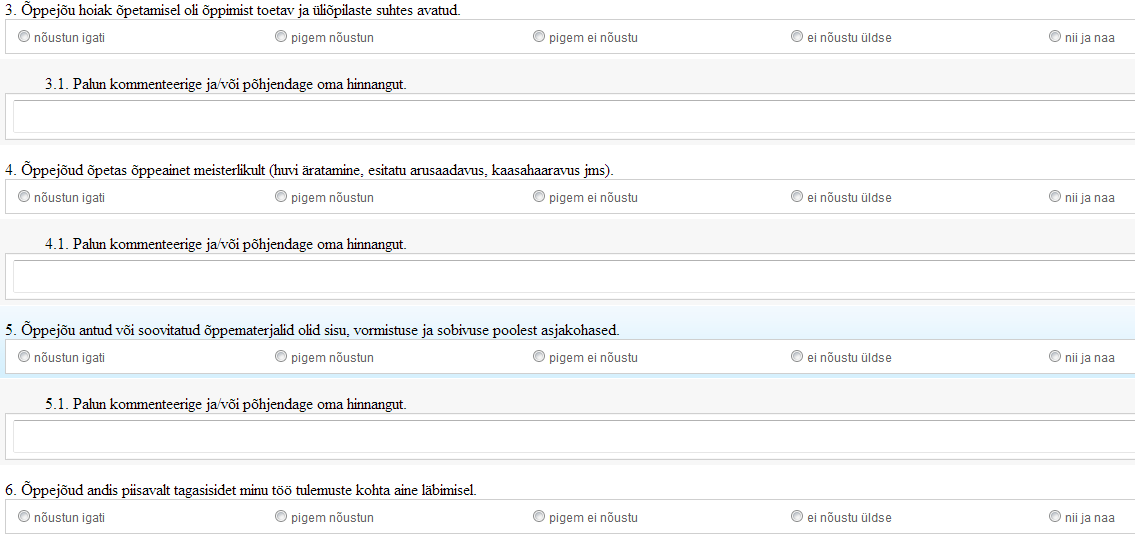
\includegraphics[width=0.8\textwidth]{ois_tagasiside_toodeldud.png}
\caption{Näide Tartu \"Ulikooli õppeinfo s\"usteemi tagasiside ankeedist, kus rakendatakse Likerti skaalat \cite{UT}}
\label{likert1}
\end{figure}

\begin{figure}[H]
\centering
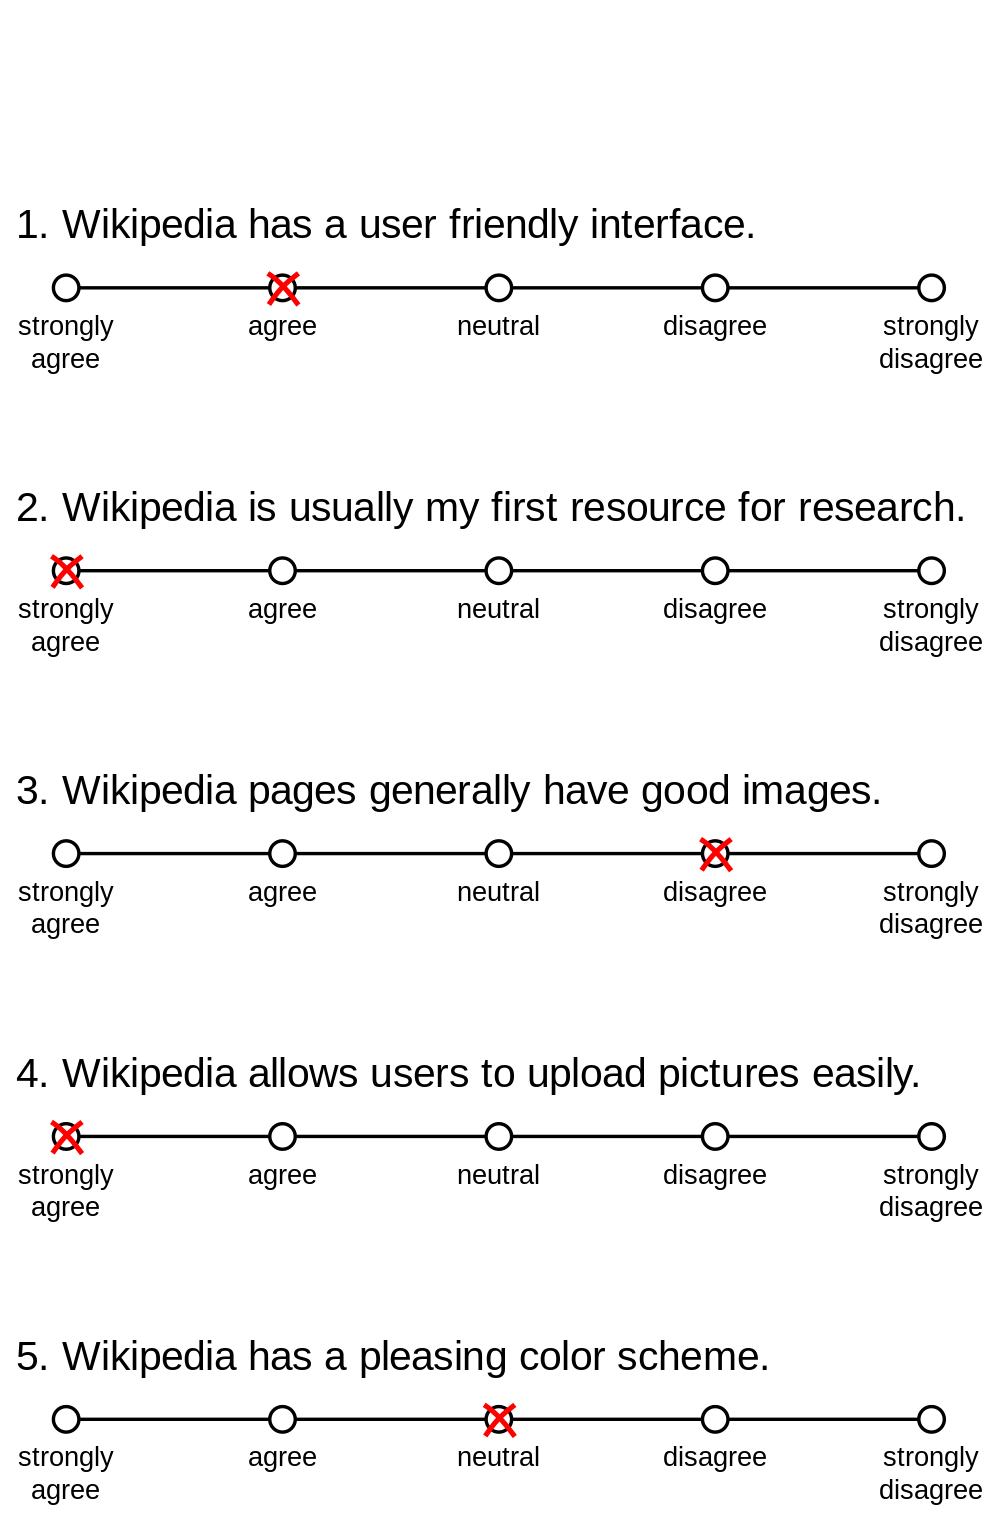
\includegraphics[width=0.5\textwidth, height = 0.7\textwidth]{Example_Likert_Scale.png}
\caption{Näide k\"usimustikust, kus on rakendatud Likerti skaalat; k\"usimused on paigutatud nende järjestikulisuse rõhutamiseks teljele\cite{Smith}}
\label{likert2}
\end{figure}



\pagebreak
\bibliography{mata_baka}{}
\bibliographystyle{plain}


\end{document}